\documentclass[main.tex]{subfiles}
\begin{document}

% ── Section A: Theory ──────────────────────────────────────────────────
\section{de Chaisemartin \& D'Haultf\oe{}uille (2020 \& 2024)}

% ── A1: Bridge from the entry slides ────────────────────────────────────
\begin{frame}{What Callaway \& Sant'Anna Assume}

  Callaway \& Sant'Anna handle the staggered binary case: an absorbing 0/1
  treatment, identified from never- and not-yet-treated controls.

  \medskip
  However, many designs do not fit that framework:
  \begin{itemize}
    \item \textbf{Non-binary treatment.} The treatment takes several values
      (a count, an intensity, a continuous dose), so ``treated versus
      untreated'' is no longer the relevant contrast.
    \item \textbf{Non-absorbing treatment.} The treatment can switch on and off,
      or rise and fall, so there is no clear and unchanged date at which a unit becomes
      treated
  \end{itemize}

 

\end{frame}

% ── A2: The intensity problem ────────────────────────────────────────────
\begin{frame}{The Non-Binary Problem: Who Is the Control?}

  When the treatment takes several values, ``treated versus untreated'' stops
  being a well-defined contrast.

  \medskip
  \begin{columns}[T]
    \begin{column}{0.46\textwidth}
      \begin{block}{Three counties, one change}
        \footnotesize
        In 2010 county B goes from $2$ to $4$ branching laws. County A has had
        $0$ all along; county C has had $2$ all along.

        \smallskip
        The change to subtract from B's is C's: C starts where B started, so
        $\Delta Y_B - \Delta Y_C$ isolates the two extra laws.

        \smallskip
        A is the wrong benchmark: a county that never had a law can sit on a
        different trend from counties that have lived with two for years.
      \end{block}
    \end{column}
    \begin{column}{0.50\textwidth}
      \textbf{What a usable comparison needs}
      \begin{itemize}\footnotesize
        \item A control that shares the treated unit's \emph{starting point},
          so the only thing separating them is the change itself.
        \item ``Untreated'' cannot deliver that when the treatment is a count
          or an intensity. There may be no untreated unit anywhere in the panel.
      \end{itemize}

      \smallskip
      \begin{exampleblock}{\footnotesize Why C\&S does not solve it}
        \footnotesize
        It is built for a binary indicator with one first-treatment date per
        unit. A dose enters only binarized, which discards it, as C\&S
        note.
      \end{exampleblock}
    \end{column}
  \end{columns}

  \medskip
  \footnotesize dCH answers by matching on the \emph{baseline dose}: the control
  for a group leaving $D=2$ is another group still sitting at $D=2$. That is the
  subject of the next few slides.

\end{frame}

% ── A3: The non-absorbing problem ────────────────────────────────────────
\begin{frame}{The Non-Absorbing Problem: No Cohorts}

  C\&S assumes treatment is permanent once adopted
  ($D_{i,t-1}=1 \Rightarrow D_{i,t}=1$). When treatment can switch off again,
  that assumption fails and the cohort idea stops working.

  \bigskip
  \begin{columns}[T]
    \begin{column}{0.48\textwidth}
      With reversible treatment the whole path matters: a unit treated in some
      periods and untreated in others has no single first-treatment date, so the
      C\&S cohort variable is undefined.
    \end{column}
    \begin{column}{0.48\textwidth}
      TWFE does not solve it either. It assumes the outcome depends only on the
      current treatment, so once past treatment still affects the outcome the
      estimate is biased, even when the treatment is binary.
    \end{column}
  \end{columns}

  \bigskip
  \begin{block}{The dCH approach}
    Date each group by its first treatment change $F_g$ (on or off, up or
    down) and compare its outcome change since $F_g-1$ with groups that had
    the same period-1 treatment and have not changed yet.
  \end{block}

\end{frame}

% ── A3b: Two dCH papers — static (2020) vs dynamic (2024) ────────────────
\begin{frame}{Two dCH Papers: Static (2020) vs.\ Dynamic (2024)}

  \textbf{``dCH'' is really two papers. Know which one you are using.}

  \medskip
  \begin{columns}[T]
    \begin{column}{0.50\textwidth}
      \begin{block}{dCH (2020, \textit{AER})}
        \footnotesize
        \textbf{Static}: the \emph{instantaneous} effect, in the period
        treatment changes.\\[3pt]
        The potential outcome is $Y_{g,t}(d)$, a \emph{single} value. That is
        where \alert{no-carryover} sits: not a separate assumption to look up,
        but the consequence of indexing by one number instead of by a path.
      \end{block}

      \smallskip
      \begin{block}{dCH (2024, \textit{REStat})}
        \footnotesize
        \textbf{Dynamic}, the version we use: $Y_{g,t}(d_1,\dots,d_t)$, indexed
        by the whole treatment path.\\[3pt]
        The estimand is the actual outcome against having kept the baseline
        dose throughout, so it \textbf{accumulates} with $\ell$.
      \end{block}
    \end{column}
    \begin{column}{0.46\textwidth}
      \textbf{Why lagged effects matter:}
      \begin{itemize}\footnotesize
        \item A hurricane hits once, and the county is back at $D=0$ the next
          year.
        \item Under the 2020 notation that county is indistinguishable from one
          never hit, so it can serve as a \emph{control} for a county hit that
          year.
        \item If the damage persists, the control is contaminated and the
          comparison is biased.
      \end{itemize}

      \smallskip
      \begin{exampleblock}{\footnotesize The same design, later today}
        \footnotesize
        Deryugina (Case~2) is exactly this: binary and non-absorbing, with
        estimated effects that keep rising from the hurricane year to five
        years later.
      \end{exampleblock}
    \end{column}
  \end{columns}

\end{frame}

% ── A3c: Set-up — what is a group? ───────────────────────────────────────
\begin{frame}{Set-Up: Groups, Periods, and Treatment}

  \textbf{The framework:} $G$ groups observed over $T$ periods, with
  outcome $Y_{g,t}$ and treatment $D_{g,t} \geq 0$.

  \medskip
  \begin{columns}[T]
    \begin{column}{0.52\textwidth}
      \begin{block}{What is a ``group'' $g$?}
        \small
        The unit whose outcome you follow, with \emph{one} treatment value
        per group and period. It can be \alert{either}:
        \begin{itemize}\small
          \item a single \textbf{individual unit} (a firm, a person)
            tracked over time, \textbf{or}
          \item a \textbf{group of individuals} (a county, a state),
            then $Y_{g,t}$ is the group's average outcome.
        \end{itemize}
        The mechanics are the same either way.
      \end{block}
    \end{column}
    \begin{column}{0.44\textwidth}
      \textbf{Treatment assigned above the unit:}
      \begin{itemize}\small
        \item State law, county data: $g$ = county or state; with
          $g$ = state, a state weighs its number of counties.
        \item $g$ = county, \texttt{cluster(state)}: clusters
          can be coarser than $g$, not finer.
      \end{itemize}

      \smallskip
      \begin{block}{\footnotesize Baseline treatment $D_{g,1}$}
        \footnotesize
        The treatment level in the \emph{first observed period}.
        It need \textbf{not} be zero, and groups are compared
        only to others with the \emph{same} $D_{g,1}$.\\[3pt]
        Starting treated is fine if pre-sample treatment has no lasting
        effect; if it lasts $\le k$ periods, start at $k{+}1$ with groups
        unchanged so far (WA~\S1.8).
      \end{block}
    \end{column}
  \end{columns}

\end{frame}

% ── A4b: Timing of a switch (moved before switchers/stayers) ─────────────
\begin{frame}{The Timing of a Switch: $F_g$, Baseline, and Horizon $\ell$}

  \textbf{Everything is dated relative to each group's own first switch.}

  \medskip
  \begin{columns}[T]
    \begin{column}{0.48\textwidth}
      \begin{block}{Three dates}
        \footnotesize
        \begin{itemize}\footnotesize
          \item $F_g = \min\{t\geq 2 : D_{g,t}\neq D_{g,t-1}\}$:
            the \textbf{first period treatment changes}.
          \item $F_g-1$: the \textbf{baseline} (last pre-switch period).
          \item $F_g-1+\ell$: the period \textbf{$\ell$ horizons after}
            the switch, where the effect at horizon $\ell$ is measured.
        \end{itemize}
      \end{block}
% aqui los em dashes confunden en mi opinion
      \smallskip
      \begin{block}{\footnotesize How far can $\ell$ go? ($T_g$)}
        \footnotesize
        $T_g$ = last period for which a same-baseline group still
        exists that has \emph{not} switched. Group $g$ enters the event
        study only up to $\ell = T_g - F_g + 1$.
      \end{block}
    \end{column}
    \begin{column}{0.48\textwidth}
      \textbf{Example: a group switching $0\to 2$ at $F_g=4$}

      \smallskip
      \footnotesize
      \begin{tabular}{@{}lcccccc@{}}
        \toprule
        $t$ & 1 & 2 & 3 & 4 & 5 & 6 \\
        $D_{g,t}$ & 0 & 0 & 0 & 2 & 2 & 2 \\
        \midrule
        role & & & base & $\ell{=}1$ & $\ell{=}2$ & $\ell{=}3$ \\
        \bottomrule
      \end{tabular}

      \smallskip
      Baseline $=F_g-1=3$; switch at $F_g=4$.\\[3pt]
      The effect at horizon $\ell$ compares the outcome at $F_g-1+\ell$ to the
      baseline, netting out what same-baseline not-yet-switched
      groups did over the same window.
    \end{column}
  \end{columns}

\end{frame}

% ── A4: The dCH solution — switchers and stayers ─────────────────────────
\begin{frame}{The dCH Solution: Switchers and Stayers}

  \textbf{Core idea:} date each group by its first treatment
  \emph{change} $F_g$ and follow it $\ell$ periods after.

  \bigskip
  \begin{columns}[T]
    \begin{column}{0.48\textwidth}
      \begin{block}{Switchers}
        Groups whose treatment first changes at $F_g$.\\[4pt]
        Later changes are part of their path.\\[4pt]
        \textbf{Treated group} in this comparison.
      \end{block}

      \medskip
      \begin{block}{Stayers (= not-yet-switched controls)}
        Units with the \emph{same baseline} $D_{g,1}$ that have
        \textbf{not yet switched} by the comparison period
        ($F_{g'} > F_g-1+\ell$).\\[4pt]
        They may switch \emph{later}, they just have not by the
        time we measure.\\[4pt]
        \textbf{Control group} in this comparison.
      \end{block}
    \end{column}
    \begin{column}{0.48\textwidth}
      \textbf{Why this is clean:}
      \begin{enumerate}
        \item Controls have the same baseline treatment as
          switchers, so they are directly comparable
        \item Controls have not switched yet, so their
          status-quo trend is uncontaminated
        \item Comparisons go switch by switch,
          no cohort definition needed
      \end{enumerate}

      \medskip
      \textbf{What we estimate:}\\[3pt]
      $\text{Effect}_\ell = \overline{Y}_{\text{switchers}}
        - \hat{Y}^0_{\text{stayers}}$\\[3pt]
      \footnotesize $\ell$ periods after the switch.
    \end{column}
  \end{columns}

\end{frame}

% ── A4b-ex1: valid-control examples (table) ──────────────────────────────
\begin{frame}{Same-Baseline Controls: Which Path Is a Valid Comparison?}

  \textbf{The control matches your \emph{baseline level}, not ``untreated.''
  Rises, falls, and returning to baseline are all valid.}

  \smallskip
  \begin{center}
  \small
  \renewcommand{\arraystretch}{1.15}
  \begin{tabular}{@{}llll@{}}
    \toprule
    \textbf{Path} & \textbf{Baseline} & \textbf{Valid control} & \textbf{Admissible?} \\
    \midrule
    $0,1,1,1$         & $0$          & baseline-$0$, not-yet-switched          & {\color{green!55!black}\checkmark}\ absorbing \\
    $0,2,2,2$         & $0$          & baseline-$0$, not-yet-switched          & {\color{green!55!black}\checkmark}\ intensity \\
    $0,2,0$\ (pulse)  & $0$          & baseline-$0$, not-yet-switched          & {\color{green!55!black}\checkmark}\ reverts, no cross \\
    $2,3,3$           & $\mathbf{2}$ & \textbf{baseline-$2$}, not-yet-switched & {\color{green!55!black}\checkmark}\ same-base $\neq$ untreated \\
    $2,1,1,1$         & $2$          & baseline-$2$, not-yet-switched          & {\color{green!55!black}\checkmark}\ de-treatment (falls) \\
    \bottomrule
  \end{tabular}
  \end{center}

  \smallskip
  \scriptsize
  \begin{itemize}\itemsep2pt
    \item \textbf{$2,3,3$:} controls are the groups \emph{still at 2}. That is the key
      innovation (match on the baseline \emph{level}, not on ``untreated'').
    \item \textbf{$0,2,0$:} the group returns to baseline, yet the effect is still the
      \emph{whole path vs.\ staying at 0}, and dCH keeps tracking the lingering effect.
    \item \textbf{$2,1,1,1$:} a switch \emph{down} (de-treatment): controls are the
      groups still at $2$; the effect is that of \emph{leaving} the dose vs.\ staying at
      $2$ (sign $S_g=-1$). Only \emph{crossing} the baseline is ruled out. See the
      No-Crossing slide.
  \end{itemize}

\end{frame}

% ── A4b-ex2: timelines (pulse + Tg) ──────────────────────────────────────
\begin{frame}{Reading the Control Period by Period}

  \textbf{(a) A transitory pulse $0\to2\to0$, and you still estimate the whole path:}
  \begin{center}\small
  \renewcommand{\arraystretch}{1.2}
  \begin{tabular}{l|cccc}
    $t$ & 1 & 2 & 3 & 4 \\
    \midrule
    \textbf{Switcher} ($F_g{=}2$) & $0$ {\scriptsize base} & $2$ {\scriptsize$(\ell{=}1)$} & $0$ {\scriptsize$(\ell{=}2)$} & $0$ {\scriptsize$(\ell{=}3)$} \\
    \textbf{Control}              & $0$ & $0$\,{\color{green!55!black}\checkmark} & $0$\,{\color{green!55!black}\checkmark} & $0$\,{\color{green!55!black}\checkmark} \\
  \end{tabular}
  \end{center}
  \footnotesize At $\ell{=}2,3$ the treatment is back at $0$, but the effect is the
  \emph{whole path vs.\ staying at 0}: the \emph{lingering} effect of the pulse.
  The control stays baseline-$0$ throughout.

  \medskip
  \normalsize\textbf{(b) How far can $\ell$ go? The control runs out:}
  \begin{center}\small
  \renewcommand{\arraystretch}{1.2}
  \begin{tabular}{l|ccccc}
    $t$ & 1 & 2 & 3 & 4 & 5 \\
    \midrule
    \textbf{Switcher} ($F_g{=}4$) & $1$ & $1$ & $1$ {\scriptsize base} & $2$ {\scriptsize$(\ell{=}1)$} & $2$ {\scriptsize$(\ell{=}2)$} \\
    \textbf{Control}              & $1$ & $1$ & $1$ & $1$\,{\color{green!55!black}\checkmark} & $\mathbf{2}$\,{\color{AlertRed}$\times$} \\
  \end{tabular}
  \end{center}
  \footnotesize $\ell{=}1$ is estimable (control still at $1$); $\ell{=}2$ is \alert{not}
  (the control has switched). $\Rightarrow T_g=4,\ \ell_{\max}=T_g-F_g+1=1$.

\end{frame}

% ── A4c: What we estimate — actual vs status quo ─────────────────────────
\begin{frame}{What We Estimate: Actual vs.\ Status Quo}

  \begin{columns}[T]
    \begin{column}{0.52\textwidth}
      \begin{defbox}{$\delta_{g,\ell}$, the actual-versus-status-quo effect (p.~5)}
        \footnotesize
        \[
          \delta_{g,\ell} = \mathbb{E}\big[\, Y_{g,F_g-1+\ell}
            - Y_{g,F_g-1+\ell}(\underbrace{D_{g,1},\ldots,D_{g,1}}_{\text{status quo}})
            \mid D \,\big]
        \]
        For group $g$, $\ell$ periods after its last pre-switch period $F_g-1$: the
        outcome under its actual dose path minus the outcome had it
        \emph{kept its baseline} dose $D_{g,1}$ throughout. The part of the
        group's evolution that is due to the change in dose.
      \end{defbox}

      \smallskip
      \textit{\small ``Versus status quo'' $=$ compared to ``keep doing
      what you were doing,'' not to ``never treated.''}
    \end{column}
    \begin{column}{0.44\textwidth}
      \begin{alertblock}{The switchers' / planner's view}
        \footnotesize
        The estimand is \textbf{conditional on the realized design}
        $D$ (like a LATE).\\[4pt]
        The effects you estimate are those of the groups that actually
        switched.\\[4pt]
        If no group with a given baseline ever switches, there is nothing to
        compare for it: the parameter is defined by the groups that moved.
      \end{alertblock}
    \end{column}
  \end{columns}

\end{frame}

% ── A6: The output — event study (moved up: the payoff picture) ──────────
\begin{frame}{The Event Study: $\delta_\ell$}

  \begin{columns}[T]
    \begin{column}{0.44\textwidth}
      \begin{tikzpicture}[scale=0.66]
        \draw[->] (-3.2,0) -- (5.5,0)
          node[right,font=\tiny] {$\ell$};
        \draw[->] (0,-0.8) -- (0,1.5)
          node[above,font=\tiny] {$\delta_\ell$};
        \draw[dashed,DarkBlue] (0,-0.8) -- (0,1.5);
        \node[below,DarkBlue,font=\tiny] at (0,-0.9) {switch};
        \foreach \x/\y in {-3/0.04,-2/-0.03,-1/0.05}{
          \fill[MidBlue] (\x,\y) circle (2.5pt);
          \draw[MidBlue,thick] (\x,\y-0.12) -- (\x,\y+0.12);
        }
        \foreach \x/\y in {1/0.10,2/0.22,3/0.38,4/0.58,5/0.80}{
          \fill[AlertRed] (\x,\y) circle (2.5pt);
          \draw[AlertRed,thick] (\x,\y-0.12) -- (\x,\y+0.12);
        }
        \node[MidBlue,font=\tiny,text width=1.6cm,align=center] at (-2,-0.42)
          {placebos $\approx 0$};
        \node[AlertRed,font=\tiny,text width=1.4cm,align=center] at (3.8,1.1)
          {$\delta_\ell$ grows};
      \end{tikzpicture}

      \footnotesize
      One number per horizon $\ell = 1, \ldots, L$. Groups are aligned by time
      since their own switch, so the same $\ell$ mixes calendar years.
      $N_\ell$ falls with $\ell$: $g$ counts only while
      $F_g-1+\ell \le T_g$, so late switchers and groups whose same-baseline
      controls have all switched drop out. Each $\delta_\ell$ averages a
      different set of groups.
    \end{column}
    \begin{column}{0.54\textwidth}
      \begin{defbox}{$\delta_\ell$, the event-study effect at horizon $\ell$ (p.~6, eq.~2)}
        \footnotesize
        $S_g = +1$ if the first change raises the dose, $-1$ if it lowers it.
        $N_\ell$: switchers that still have a not-yet-switched
        same-baseline control, $F_g - 1 + \ell \le T_g$.
        \[
          \delta_\ell = \frac{1}{N_\ell}\sum_{g:\, F_g-1+\ell \le T_g} S_g\, \delta_{g,\ell}
        \]
        The average of $\delta_{g,\ell}$ over the groups still observed at
        horizon $\ell$, switchers whose dose fell entering with the sign
        flipped: the effect of having received a weakly higher dose for
        $\ell$ periods.
      \end{defbox}

      \smallskip
      \footnotesize Example, $\ell = 3$: A switched in 1996 and contributes
      its 1998 effect, B switched in 1999 and contributes its 2001 effect; a
      group that switched in 2004 in a panel ending in 2005 is not in $N_3$.
    \end{column}
  \end{columns}

\end{frame}

% ── A6b: placebos and path-specific effects ──────────────────────────────
\begin{frame}{Placebos and Path-Specific Effects}

  \begin{columns}[T]
    \begin{column}{0.50\textwidth}
      \begin{defbox}{$\delta^{pl}_\ell$, the placebo at horizon $\ell$ (p.~11)}
        \footnotesize
        The same construction as $\delta_\ell$ on the $\ell$ periods
        \emph{before} the switch: the change $Y_{g,F_g-1-\ell} - Y_{g,F_g-1}$
        of the switchers against the same change of their controls. Under no
        anticipation and parallel trends its expectation is zero. It tests
        parallel trends over as many periods as $\delta_\ell$ needs ($\ell$),
        with the same controls, but before the switch, not after it.
      \end{defbox}
    \end{column}
    \begin{column}{0.46\textwidth}
      \begin{defbox}{path-specific $\delta_\ell$ (pp.~6--7, fn.~10)}
        \footnotesize
        The average in $\delta_\ell$ restricted to the groups that share the
        same dose path $(D_{g,1}, D_{g,F_g}, \ldots, D_{g,F_g-1+\ell})$: one
        event study per path. Useful when a few paths cover most switchers;
        each path then has fewer groups.
      \end{defbox}
    \end{column}
  \end{columns}

  \medskip
  \footnotesize Three levels of the same object. $\delta_{g,\ell}$: one group,
  one horizon. Path-specific $\delta_\ell$: the groups that did the same
  thing. $\delta_\ell$: all the groups observed at that horizon.

\end{frame}

% ── A4d: The DID_{g,l} estimator formula ─────────────────────────────────
\begin{frame}{The $\text{DID}_{g,\ell}$ Estimator}

  \footnotesize
  $\delta_{g,\ell}$ is the estimand, never observed. $\text{DID}_{g,\ell}$ is
  the estimator, built from changes seen in the data; Lemma~1 links the two.

  \begin{defbox}{$\text{DID}_{g,\ell}$, the estimator of $\delta_{g,\ell}$ (p.~5)}
  \small
  \[
    \text{DID}_{g,\ell}
      = \underbrace{\big[Y_{g,F_g-1+\ell} - Y_{g,F_g-1}\big]}_{\text{switcher } g\text{'s change}}
      - \underbrace{\frac{1}{N^g_{F_g-1+\ell}}\!\!\!\sum_{\substack{g':\, D_{g',1}=D_{g,1}\\ F_{g'} > F_g-1+\ell}}\!\!\!\big[Y_{g',F_g-1+\ell} - Y_{g',F_g-1}\big]}_{\text{same-baseline, not-yet-switched controls}}
  \]
  \end{defbox}

  \medskip
  \begin{columns}[T]
    \begin{column}{0.52\textwidth}
      \begin{itemize}\footnotesize
        \item Term 1: $g$'s outcome change from baseline $F_g-1$ to
          horizon $F_g-1+\ell$.
        \item Term 2: the average change over the \emph{same window}
          among controls with the \textbf{same baseline} $D_{g,1}$
          that have \textbf{not switched} by $F_g-1+\ell$.
        \item $N^g_t$ = number of such controls.
      \end{itemize}
    \end{column}
    \begin{column}{0.44\textwidth}
      \begin{block}{\footnotesize The key innovation}
        \footnotesize
        Controls match on the \emph{baseline level}, not on
        ``untreated.'' Groups all at $D{=}2$ in period 1 form their
        own comparison set.
      \end{block}

      \smallskip
      \begin{exampleblock}{\footnotesize Unbiasedness (Lemma 1)}
        \footnotesize
        Under no-anticipation $+$ parallel trends on the status-quo
        outcome, $\mathbb{E}[\text{DID}_{g,\ell}\mid D]=\delta_{g,\ell}$.
      \end{exampleblock}
    \end{column}
  \end{columns}
\end{frame}

% ── A5: Key assumptions ───────────────────────────────────────────────────
\begin{frame}{Key Assumptions}

  \begin{columns}[T]
    \begin{column}{0.50\textwidth}
      \begin{block}{(a) Parallel trends on the \emph{status-quo} outcome}
        Among groups with the same baseline $D_{g,1}$, the \emph{status-quo}
        outcome (``keep $D_{g,1}$'') evolves in parallel in every period
        (A2, p.~5).\\[6pt]
        Weaker than parallel trends across \emph{different} baselines
        (A3, p.~7), which rules out lagged and time-varying effects; A2
        leaves them free.
      \end{block}

      \medskip
      \begin{block}{(b) No anticipation}
        No outcome depends on future treatments:
        $Y_{g,t}(d_1,\dots,d_T)=Y_{g,t}(d_1,\dots,d_t)$ (A1, p.~5).\\[6pt]
        Enables pre-treatment placebo tests.
      \end{block}
    \end{column}
    \begin{column}{0.46\textwidth}
      \begin{block}{(c) Lagged effects are \textbf{allowed}}
        $Y_{g,t}$ may depend on the \emph{full treatment history}, so lagged
        exposure, learning, habit formation.\\[4pt]
        This is the key advantage for non-absorbing designs, where past
        treatment plausibly still shapes today's outcome.
      \end{block}

      \smallskip
      \begin{alertblock}{Design requirement}
        \footnotesize
        Some baseline level must contain groups that switch at
        \emph{different} dates (design restriction 1, p.~4); baseline
        levels without such a pair contribute nothing. If all units
        switch simultaneously, identification fails.
      \end{alertblock}
    \end{column}
  \end{columns}

\end{frame}

% ── A5b: No-crossing condition ───────────────────────────────────────────
\begin{frame}{The No-Crossing Condition}

  \textbf{Design restriction 2 (p.~6):} each group's treatment must stay on \emph{one
  side} of its baseline: either $D_{g,t}\geq D_{g,1}$ for all $t$
  (only rises), or $D_{g,t}\leq D_{g,1}$ for all $t$ (only falls).
  It must never cross back over $D_{g,1}$.

  \medskip
  \begin{columns}[T]
    \begin{column}{0.50\textwidth}
      \begin{alertblock}{Why crossing breaks things}
        \footnotesize
        A group with path $2,3,1$ (baseline $2$) goes \emph{above}
        ($3$) then \emph{below} ($1$) its baseline. Its $\delta_{g,\ell}$
        can then be written with \alert{negative weights} and may flip
        sign even if every true effect is monotone, violating
        no-sign-reversal.
      \end{alertblock}

      \smallskip
      \textit{\footnotesize Intuition: the estimator nets effects
      against the baseline. If a group wanders to both sides, the
      above- and below-baseline effects get tangled with opposing
      signs.}
    \end{column}
    \begin{column}{0.46\textwidth}
      \begin{block}{When it holds automatically}
        \footnotesize
        \begin{itemize}\footnotesize
          \item Binary treatment
          \item A single treatment change
          \item $D_{g,1}=0$ for all groups
        \end{itemize}
      \end{block}

      \smallskip
      \begin{block}{\footnotesize If violated}
        \footnotesize
        The cells where $g$ has been both strictly above and strictly below
        its baseline are dropped (fn.~8, p.~6).
      \end{block}
    \end{column}
  \end{columns}

\end{frame}

% ── A6b: Switchers-in vs switchers-out ───────────────────────────────────
\begin{frame}{Switchers-In vs.\ Switchers-Out}

  \textbf{Switchers come in two kinds, by the \emph{direction} of the first
  change.}

  \medskip
  \begin{columns}[T]
    \begin{column}{0.52\textwidth}
      \begin{block}{The sign of the switch}
        \[
          S_g = \mathbf{1}\{D_{g,F_g}>D_{g,1}\} - \mathbf{1}\{D_{g,F_g}<D_{g,1}\}
        \]
        \footnotesize
        $S_g=+1$: \textbf{switcher-in} (dose rises above baseline).\\
        $S_g=-1$: \textbf{switcher-out} (dose falls below baseline).
      \end{block}

      \smallskip
      \begin{defbox}{$\text{DID}_\ell$, the estimator of $\delta_\ell$ (p.~6; companion eq.~5)}
        \footnotesize
        Two event studies, $\text{DID}_{+,\ell}$ over the $N^1_\ell$
        switchers-in and $\text{DID}_{-,\ell}$ over the $N^0_\ell$
        switchers-out (built on $-\text{DID}_{g,\ell}$), then aggregated:
        \[
          \text{DID}_\ell = \tfrac{N^1_\ell}{N^1_\ell+N^0_\ell}\text{DID}_{+,\ell}
            + \tfrac{N^0_\ell}{N^1_\ell+N^0_\ell}\text{DID}_{-,\ell}.
        \]
      \end{defbox}
    \end{column}
    \begin{column}{0.44\textwidth}
      \begin{exampleblock}{Why flip the sign for switchers-out?}
        \footnotesize
        After the flip, \emph{every} term reads as ``the effect of being
        exposed to a \textbf{weakly larger dose} for $\ell$ periods.''
        Ins and outs are placed on the same footing, so $\text{DID}_\ell$
        aggregates comparable quantities.
      \end{exampleblock}

      \smallskip
      \begin{alertblock}{Pooling ins and outs}
        \footnotesize
        $\text{DID}_\ell$ averages the effect of adding dose with the
        sign-flipped effect of removing it. If they may differ (a plant
        closing hurts more than its opening lifts), estimate them
        \textbf{separately}: \texttt{switchers(in)}, \texttt{switchers(out)}.
      \end{alertblock}
    \end{column}
  \end{columns}

\end{frame}

% ── A7: The dose accumulated, delta^D (p. 7) ─────────────────────────────
\begin{frame}{The Dose Accumulated: $\delta^{D}_{g,\ell}$ and $\delta^{D}_\ell$}

  \textbf{With a non-binary treatment, $\delta_\ell$ averages groups whose extra
  dose differs in size and in duration} (p.~6): a $0\!\to\!1$ switch and a
  $0\!\to\!4$ switch enter as one switcher each. To compare them the effect
  is divided by the amount of treatment received (p.~7).

  \medskip
  \begin{columns}[T]
    \begin{column}{0.54\textwidth}
      \begin{defbox}{$\delta^{D}_{g,\ell}$, the dose accumulated up to horizon $\ell$ (pp.~7--8)}
        \footnotesize
        \[
          \delta^{D}_{g,\ell} = \sum_{k=0}^{\ell-1}\big(D_{g,F_g+k}-D_{g,1}\big),
          \qquad
          \delta^{D}_\ell = \frac{1}{N_\ell}\sum_{g:\, F_g-1+\ell \le T_g} \big|\delta^{D}_{g,\ell}\big|
        \]
        Every dose-period received from the switch to $F_g-1+\ell$, summed;
        and its average over the switchers observed at $\ell$. A quantity of
        treatment, computed from $D$, with no estimation error.
      \end{defbox}
    \end{column}
    \begin{column}{0.42\textwidth}
      \begin{block}{\footnotesize The unit: a dose-period}
        \footnotesize
        One unit of $D$ in force during one period. A binary policy: one
        period under the policy. A count of laws: a law-year. A share in
        points: a point-year.
      \end{block}

      \smallskip
      \footnotesize A group that goes from $0$ to $2$ and stays: in force
      $2, 2, 2$; accumulated $2, 4, 6$. If it moves to $3$ in its third
      period: $2, 4, 7$. Binary absorbing: accumulated $= \ell$.
    \end{column}
  \end{columns}

\end{frame}

% ── A7a: Normalized effects (dCH 2024, Lemma 2) ──────────────────────────
\begin{frame}{The Normalized Effect: $\delta^{n}_{g,\ell}$ and $\delta^{n}_\ell$}

  \begin{columns}[T]
    \begin{column}{0.50\textwidth}
      \begin{defbox}{$\delta^{n}_{g,\ell}$ and $\delta^{n}_\ell$, the effect per dose-period (pp.~7--8, eq.~4)}
        \footnotesize
        \[
          \delta^{n}_{g,\ell} = \frac{\delta_{g,\ell}}{\delta^{D}_{g,\ell}},
          \qquad
          \delta^{n}_\ell = \frac{\delta_\ell}{\delta^{D}_\ell}
        \]
        The effect divided by the dose accumulated up to $\ell$: what one
        dose-period has added by horizon $\ell$, in outcome units per
        dose-period, comparable across groups whatever their dose.
      \end{defbox}
    \end{column}
    \begin{column}{0.46\textwidth}
      \begin{block}{\footnotesize Lemma 2 (p.~8): what it averages}
        \footnotesize
        \[
          \delta^{n}_{g,\ell} = \sum_{k=0}^{\ell-1} w_{g,\ell,k}\, s_{g,\ell,k}
        \]
        a weighted average of the slopes (effect per unit of dose) with
        respect to the current dose ($k=0$) and its $\ell-1$ lags, with
        weights $w_{g,\ell,k}$ proportional to the extra dose at each lag,
        summing to one and non-negative under design restriction~2. One
        change kept in force: $1/\ell$ each.
      \end{block}
    \end{column}
  \end{columns}

  \medskip
  \footnotesize The lags cannot be separated unless lag effects are additive,
  linear and constant over time (fn.~15); the weights $w_{\ell,k}$ can be
  reported (p.~9). A flat profile $\ell \mapsto \delta^{n}_\ell$ says current
  and lagged doses have similar effects (p.~17); with one change kept in
  force, a profile falling as $1/\ell$ says only the dose in force matters.

\end{frame}

% ── A7w: in words (1), from the raw effect to the normalized effect ──────
\begin{frame}{In Words (1): From the Raw Effect to the Normalized Effect}

  \footnotesize
  \textbf{Raw.} $\delta_{g,\ell}$ is the group's actual outcome against its
  status quo, $\ell$ periods after the switch; $\delta_\ell$ is the same
  thing averaged over the switchers observed at $\ell$. With a binary
  absorbing treatment nothing more is needed: every switcher took the same dose, one
  unit.

  \medskip
  \textbf{Why a non-binary treatment needs more.} Switchers differ in how much
  dose they took, and the dose stays in force period after period, so the
  effect measured at $\ell$ reflects both how much and for how long.
  $\delta_\ell$ averages a $0\!\to\!1$ county and a $0\!\to\!4$ county as one
  switcher each.

  \medskip
  \textbf{Accumulated dose.} $\delta^{D}_{g,\ell}$ counts the dose-periods the
  group has received since its switch: $0 \to 2$ and staying gives $2, 4, 6$.
  $\delta^{D}_\ell$ is the \emph{average} of those counts over the switchers
  observed at $\ell$, an average like $\delta_\ell$, not a sum. A second
  county that moves $0 \to 1$ one period later has $1, 2$ at its own
  $\ell = 1, 2$ and is not observed at $\ell = 3$: $\delta^{D}_\ell$ is
  $(2+1)/2 = 1.5$, then $(4+2)/2 = 3$, then $6$.

  \medskip
  \textbf{Normalized.} $\delta^{n}_\ell = \delta_\ell / \delta^{D}_\ell$, the
  raw effect divided by the accumulated dose: the effect per dose-period.
  Numerator and denominator average over the same groups, so it also equals
  the sum of the groups' sign-adjusted effects $S_g\delta_{g,\ell}$ over the
  sum of their absolute dose-periods $|\delta^{D}_{g,\ell}|$, and it is a
  $|\delta^{D}_{g,\ell}|$-weighted average of each group's own
  $\delta_{g,\ell} / \delta^{D}_{g,\ell}$ (eq.~4).

\end{frame}

% ── A7b: The average total effect per unit of treatment (p. 9) ───────────
\begin{frame}{The Average Total Effect per Unit of Treatment, $\delta$}

  \begin{columns}[T]
    \begin{column}{0.52\textwidth}
      \begin{defbox}{$\delta$, the average total effect per unit of treatment (p.~9)}
        \scriptsize
        \[
          \delta = \frac{\sum_{g}\sum_{\ell=1}^{T_g-F_g+1} \delta_{g,\ell}}
                        {\sum_{g}\sum_{\ell=1}^{T_g-F_g+1} \big(D_{g,F_g-1+\ell}-D_{g,1}\big)}
        \]
        Every actual-versus-status-quo effect, over every horizon a switcher
        is observed, divided by every dose-period in force over those
        horizons: the total effect of one dose-period, the period it arrives
        and every later horizon in the window. No subscript, as in the paper:
        one number over all groups and horizons.
      \end{defbox}

      \smallskip
      \footnotesize With no discounting and a cost linear in the dose, the
      switchers' actual treatments are beneficial iff $\delta > c$, the
      average cost of one dose-period (p.~9). Lemma 3
      (p.~10): under design restrictions 1 and 3 (no group ever goes below
      its baseline, p.~9), $\delta = \sum_\ell w_\ell\, \delta_\ell$ with
      non-negative weights, so if every $\delta_\ell$ has the same sign,
      $\delta$ has it too.
    \end{column}
    \begin{column}{0.46\textwidth}
      \begin{defbox}{the average number of periods over which a dose's effect is cumulated (p.~10)}
        \scriptsize
        \[
          \frac{\sum_g\sum_{k=0}^{T_g-F_g}\big(D_{g,F_g+k}-D_{g,1}\big)\,(T_g-F_g-k+1)}
               {\sum_g\sum_{k=0}^{T_g-F_g}\big(D_{g,F_g+k}-D_{g,1}\big)}
        \]
        Each dose-period weighted by the number of horizons it is counted in.
        Dividing $\delta$ by it gives the average effect of one dose for one
        period.
      \end{defbox}

      \smallskip
      \footnotesize Binary staggered with a never-treated group (p.~9):
      $\delta$ is the average, over treated $(g,t)$ cells, of the effect of
      having been treated for $t-F_g+1$ periods, the ATT generalized to
      dynamic effects; and $\delta^{n}_\ell = \delta_\ell/\ell$.
    \end{column}
  \end{columns}

\end{frame}

% ── A7x: in words (2), the average total effect ──────────────────────────
\begin{frame}{In Words (2): The Average Total Effect per Unit of Treatment}

  \footnotesize
  \textbf{A sum, not a division horizon by horizon.} The numerator adds every
  raw effect $\delta_{g,\ell}$ of every switcher at every horizon it is
  observed. The denominator adds the extra dose \emph{in force} at each of
  those group-horizons: the total dose-periods received over the window. The
  county at $0 \to 2$ for three periods contributes $2+2+2 = 6$ dose-periods;
  the county at $0 \to 1$ for two periods contributes $2$; eight in all.

  \medskip
  \textbf{In force, not accumulated.} $\delta^{D}_{g,\ell}$ already contains
  the earlier periods; summing it over $\ell$ would count the first
  dose-period three times. $\delta$ sums the flow of each period, which equals
  the group's accumulated dose at its last observed horizon.

  \medskip
  \textbf{The same fraction per cell.} Divide numerator and
  denominator by the number of group-horizon cells: $\delta$ is the average
  raw effect per cell divided by the average dose in force per cell. Binary
  absorbing treatment: the dose in force is $1$, and $\delta$ is the average of the
  $\delta_\ell$ weighted by the switchers at each horizon. With a dose, the
  same average divided by the mean dose in force.

  \medskip
  \textbf{Against the normalized effect.} Both divide by dose. $\delta^{n}_\ell$
  divides one horizon's effect by the dose accumulated up to it: what a
  dose-period adds per period. $\delta$ divides all effects by all
  dose-periods, and since a dose-period keeps being counted in later horizons,
  it gives what a dose-period adds in total over the window. $\delta = M
  \times$ the average of the $\delta^{n}_\ell$ weighted by the dose
  accumulated at $\ell$, with $M$ the average number of periods over which a
  dose's effect is cumulated (p.~10; derived from Lemma~3). $\delta/M$ equals
  every $\delta^{n}_\ell$ exactly when the profile is flat.

\end{frame}

% ── A8: dCH vs. C&S comparison ───────────────────────────────────────────
\begin{frame}{dCH vs.\ C\&S: When to Use Which}

  \begin{columns}[T]
    \begin{column}{0.50\textwidth}
      \footnotesize
      \begin{tabular}{lcc}
        \toprule
        \textbf{Feature} & \textbf{C\&S} & \textbf{dCH} \\
        \midrule
        Binary treatment     & Yes & Yes \\
        Non-binary / intensity & No  & \textbf{Yes} \\
        Absorbing treatment  & Yes & Yes \\
        Non-absorbing        & No  & \textbf{Yes} \\
        Doubly robust        & \textbf{Yes} & No \\
        Covariate-adj.\ PT   & \textbf{Yes} & Linear only \\
        Default SEs (Stata)  & Analytic & Analytic \\
        \bottomrule
      \end{tabular}

      \smallskip
      \begin{block}{\footnotesize What each one requires}
        \footnotesize
        C\&S requires a binary, absorbing treatment; when all units start
        untreated, dCH's assumption~2 is similar to its parallel trends (p.~5).
        dCH allows any design satisfying restriction~1 (p.~4).

        \smallskip
        \textbf{When every unit starts untreated, $\text{DID}_\ell$ equals
        the C\&S event study at $\ell-1$ computed on the binarized and
        staggerized treatment} (dCH 2024 \textit{REStat}, p.~7).
      \end{block}
    \end{column}
    \begin{column}{0.46\textwidth}
      \textbf{Decision rule:}
      \begin{itemize}
        \item \textbf{Binary and absorbing?}\\
          Both valid. Use dCH as a robustness check
          for C\&S. If they agree, C\&S is preferred
          (doubly robust).
        \item \textbf{Non-binary (intensity/count)?}\\
          \alert{dCH only}
        \item \textbf{Non-absorbing (reversible)?}\\
          \alert{dCH only}, allowing full treatment
          history to affect $Y$
        \item \textbf{Covariates important?}\\
          C\&S has the stronger doubly-robust estimator
      \end{itemize}
    \end{column}
  \end{columns}

\end{frame}

% ── Extensions (1): relaxing parallel trends (teaser) ────────────────────
\begin{frame}{Extensions (1): Relaxing Parallel Trends}

  The baseline parallel-trends assumption can be weakened in several ways.
  Rather than list them abstractly, we introduce each \emph{in the case that
  needs it}, where a concrete failure makes the fix easy to motivate:

  \medskip
  \begin{itemize}
    \item \textbf{Covariate-adjusted} trends, \texttt{controls()}: Deryugina (Case 2).
    \item \textbf{Trends within sets of groups}, \texttt{trends\_nonparam()}: Hollingsworth (Case 5).
    \item \textbf{Group-specific linear} trends, \texttt{trends\_lin}.
    \item A smooth \textbf{polynomial} trend for a continuous baseline: next slide.
  \end{itemize}

\end{frame}

% ── Extensions (2): continuous treatment ─────────────────────────────────
\begin{frame}{Extensions (2): Continuous Treatment}

  When the period-one treatment $D_{g,1}$ is continuously distributed, no two
  groups share a baseline, so same-baseline matching has nothing to work with.

  \medskip
  \begin{columns}[T]
    \begin{column}{0.54\textwidth}
      \begin{block}{Model the trend in the baseline}
        \footnotesize
        Instead of matching on an identical $D_{g,1}$, assume the status-quo
        trend is a smooth (polynomial) function of the baseline:
        \[
          \mathbb{E}\!\left[\Delta Y_{g,t}^{\text{sq}}\mid D\right]
            = \sum_{k=0}^{K}\gamma_{k,t}\,D_{g,1}^{\,k},
        \]
        with the order $K$ chosen by the researcher. This trend is netted out,
        and the estimator proceeds as before.
      \end{block}
    \end{column}
    \begin{column}{0.42\textwidth}
      \begin{block}{\footnotesize What it identifies}
        \footnotesize
        By default, the \textbf{level} effect of having changed the dose: the
        numerator uses a binarised switch (companion, pp.~22--23). Dividing by
        the actual change in $D$, in the normalized effect and in $\delta$,
        gives an effect \textbf{per unit of dose}: a scaled level, not a
        derivative at a point.
      \end{block}

      \smallskip
      \begin{alertblock}{\footnotesize Inference}
        \footnotesize
        Variance is conservative when $K$ is right, possibly liberal when too
        high, so inference relies on the bootstrap.
      \end{alertblock}
    \end{column}
  \end{columns}

  \smallskip
  \footnotesize A topic of its own, developed in later work (de Chaisemartin,
  D'Haultf\oe{}uille, Pasquier \& Vazquez-Bare 2022; Callaway, Goodman-Bacon \&
  Sant'Anna, forthcoming \textit{AER}). We use the dCH option for it in Case~3,
  and take up the question properly in the continuous-treatment block.

\end{frame}

% ── Command: the did_multiplegt_dyn package (walkthrough) ────────────────
\begin{frame}[fragile]{Running \texttt{did\_multiplegt\_dyn}: One Command, Step by Step}

\lstset{
  language={},
  basicstyle=\small\ttfamily,
  keywordstyle=\color{MidBlue},
  commentstyle=\color{gray},
  breaklines=true,
  showstringspaces=false
}

\begin{lstlisting}
* ssc install did_multiplegt_dyn   // once
did_multiplegt_dyn Y G T D, ///
    effects(8) placebo(3) cluster(state_n)
\end{lstlisting}

  \smallskip
  \begin{columns}[T]
    \begin{column}{0.5\textwidth}
      \textbf{The four arguments, left to right:}
      \begin{itemize}\footnotesize
        \item \texttt{Y}: the outcome.
        \item \texttt{G}: the group, the unit whose outcome you follow, with
          one treatment value per group and period: the \emph{county} in
          Favara, though the law is set by state; the state goes to
          \texttt{cluster()}.
        \item \texttt{T}: the time variable.
        \item \texttt{D}: the treatment.
      \end{itemize}
    \end{column}
    \begin{column}{0.5\textwidth}
      \textbf{The three base options:}
      \begin{itemize}\footnotesize
        \item \texttt{effects(8)}: the switch period and the 7 \emph{after}.
        \item \texttt{placebo(3)}: check 3 periods \emph{before}
          (must be $\le$ \texttt{effects}).
        \item \texttt{cluster(state\_n)}: SEs by state with $g$ = county;
          the default is $g$, and only a coarser level is allowed, never
          finer.
      \end{itemize}
    \end{column}
  \end{columns}

  \smallskip
  \begin{center}\tiny
  \setlength{\tabcolsep}{3pt}
  \begin{tabular}{@{}p{2.8cm}p{5.0cm}p{2.9cm}@{}}
    \toprule
    Paper & Output & Option \\
    \midrule
    $\delta_\ell$, event-study effect & \texttt{Effect\_}$\ell$, with $N$ (observations, fn.~4) and Switchers (groups) & default \\
    placebo effect & \texttt{Placebo\_}$\ell$ & \texttt{placebo(\#)} \\
    $\delta^{n}_\ell$, per dose-period (Lemma 2) & \texttt{Effect\_}$\ell$ & \texttt{normalized} \\
    lag weights $w_{\ell,k}$ & table $k \times \ell$ & \texttt{normalized normalized\_weights} \\
    $\delta$, total per dose-period (p.~9) & \texttt{Av\_tot\_eff}; also \texttt{Switch x Periods} and the average number of periods over which a dose's effect is cumulated (p.~10) & default; not with \texttt{trends\_lin} \\
    \bottomrule
  \end{tabular}
  \end{center}

\end{frame}

% ── How to read each number, in one sentence ─────────────────────────────
\begin{frame}{How to Read Each Number, in One Sentence}

  \scriptsize
  \textbf{Raw \texttt{Effect\_}$\ell$.} In the $\ell$-th period counting the
  period of their first change, so $\ell-1$ periods after it, switchers'
  outcome is on average [Effect$_\ell$] [units of $Y$] higher than had they
  kept their initial dose (``lower'' if their dose fell, $S_g=-1$, p.~6).\\
  \textit{En el periodo $\ell$ contando el de su primer cambio, es decir
  $\ell-1$ periodos después, el outcome de los switchers es en media
  [Effect$_\ell$] [unidades] mayor que con su dosis inicial (``menor'' si su
  dosis bajó).}

  \medskip
  \textbf{\texttt{Effect\_}$\ell$ with \texttt{normalized}.} At horizon $\ell$,
  each dose-period accumulated since the switch accounts for [Effect$_\ell$]
  [units of $Y$], an average over the current dose and its lags.\\
  \textit{En el horizonte $\ell$, cada dosis-periodo acumulada desde el cambio
  explica [Effect$_\ell$] [unidades], media de la dosis actual y las
  rezagadas.}

  \medskip
  \textbf{\texttt{Av\_tot\_eff}.} One unit of dose in force for one period
  changes the outcome by [Av\_tot\_eff] [units of $Y$] in total over the
  \texttt{effects()} window.\\
  \textit{Una unidad de dosis en vigor durante un periodo cambia el outcome en
  [Av\_tot\_eff] [unidades] en total a lo largo de la ventana.}

  \medskip
  \textbf{\texttt{Placebo\_}$\ell$.} In the $\ell$ periods before the change,
  switchers and their controls moved alike (joint $p = \ldots$), or apart by
  [Placebo$_\ell$].\\
  \textit{En los $\ell$ periodos anteriores al cambio, switchers y controles se
  movían igual ($p$ conjunto $= \ldots$).}

  \medskip
  \textbf{Units.} Those of $Y$: a log outcome reads in percent ($0.011
  \approx 1.1$\,\%); a dose in its own unit (law-years, newspaper-elections,
  a unit of eligibility, 100 points, for a year). Binary absorbing:
  \texttt{Effect\_}$\ell$ is the effect of $\ell$ periods under treatment,
  \texttt{normalized} divides it by $\ell$, \texttt{Av\_tot\_eff} is the
  switcher-weighted mean of the raw effects. Binary pulse, one period in
  force: \texttt{Av\_tot\_eff} sums the effects, each weighted by the share
  of switchers left at that horizon.

\end{frame}

% ── Section B: Applications ──────────────────────────────────────────────
\section{Applications}

\lstset{
  language={},
  basicstyle=\tiny\ttfamily,
  keywordstyle=\color{MidBlue},
  commentstyle=\color{gray},
  stringstyle=\color{AlertRed},
  breaklines=true,
  showstringspaces=false
}

% ── Overview: the five cases ──────────────────────────────────────────────
\begin{frame}{Five Cases}

  \textbf{One engine, matching on the baseline and comparing switchers to
  not-yet-switchers, spans a whole family of designs.}

  \medskip
  \begin{tabular}{@{}cll@{}}
    \toprule
     & \textbf{Paper} & \textbf{Treatment} \\
    \midrule
    \textbf{1} & Favara \& Imbs (2015)        & Count 0--4 (restrictions lifted) \\[4pt]
    \textbf{2} & Deryugina (2017)             & Binary non-absorbing \\[4pt]
    \textbf{3} & East et al.\ (2023)          & Continuous (Medicaid \%) \\[4pt]
    \textbf{4} & Gentzkow et al.\ (2011)      & Count (newspapers) \\[4pt]
    \textbf{5} & Hollingsworth et al.\ (2022) & Sequential binary (mm $\to$ rm) \\
    \bottomrule
  \end{tabular}

  \bigskip
  Full code: \texttt{Stata/Block2\_dCH\_practice.do}

\end{frame}

% ════════════════════════════════════════════════════════════════════════
% CASE 1: FAVARA & IMBS (2015) — Non-binary count treatment
% ════════════════════════════════════════════════════════════════════════

\begin{frame}{Case 1 --- Favara \& Imbs (2015): Context \& Data}

  \begin{columns}[T]
    \begin{column}{0.50\textwidth}
      \textbf{Research question}\\
      Does credit supply (bank branching deregulation) raise mortgage
      lending?

      \medskip
      \textbf{Paper}\\
      Favara \& Imbs (2015), \textit{AER} 105(3): 958--992.

      \medskip
      \textbf{Data} (replication package)\\
      \textbf{1{,}048 US counties} $\times$ \textbf{12 years} (1994--2005);
      12{,}538 obs; clustered by state (50).\\[3pt]
      Outcome \texttt{Dl\_vloans\_b} (log change in mortgage volume);
      treatment \texttt{inter\_bra} (interstate-branching restrictions
      lifted; reversed Rice \& Strahan index, 0--4).
    \end{column}
    \begin{column}{0.46\textwidth}
      \begin{block}{Design (read off the data)}
        \footnotesize
        \begin{itemize}\footnotesize
          \item \textbf{Count} treatment $\in\{0,1,2,3,4\}$ (Rice \&
            Strahan index).
          \item \textbf{99.9\%} of counties start at 0 (first observed year).
          \item Mostly accumulating: 1{,}056 increases vs.\ 46 decreases.
          \item \textbf{917} counties change their index; \textbf{905} enter the estimation at $\ell=1$.
        \end{itemize}
      \end{block}

      \smallskip
      \footnotesize Non-binary, so TWFE makes an intermediate-dose county both
      treated and control; dCH with \texttt{normalized} gives the effect per
      additional restriction lifted.
    \end{column}
  \end{columns}

\end{frame}

\begin{frame}[fragile]{Case 1 --- The Output, Block by Block}

  \begin{columns}[T]
    \begin{column}{0.60\textwidth}
\begin{lstlisting}[basicstyle=\tiny\ttfamily]
Estimation of treatment effects: Event-study effects
           |  Estimate       SE     LB CI     UB CI      N
  Effect_1 |  .0434814 .0354981 -.0260935  .1130563   3810   (1)
  ...
  Effect_8 |   .185827 .0794133  .0301799  .3414741   1248
           | Switchers
  Effect_1 |       905    ...    Effect_8 |    773           (2)
Test of joint nullity of the effects : p-value = .0635       (3)

Average cumulative (total) effect per treatment unit
Av_tot_eff |  .0478284 .0246733 -.0005305  .0961873  10598   (4)
           | Switch x Periods
Av_tot_eff |      6921                                       (5)
Average number of time periods over which a treatment's
  effect is accumulated = 4.3392959                          (6)

Testing the parallel trends and no anticipation assumptions
 Placebo_1 |  .0548088 .0511118 -.0453685   .154986   2777   (7)
  ...
Test of joint nullity of the placebos : p-value = .4068
\end{lstlisting}
    \end{column}
    \begin{column}{0.38\textwidth}
      \scriptsize
      \begin{enumerate}
        \item Raw Effect$_\ell$, in the outcome's units (log points of loan
          growth); with \texttt{normalized}, per law-year. $N$: observations
          used.
        \item Switchers observed $\ell$ periods after switching; the count
          falls once no same-baseline control is left.
        \item Joint test of the eight effects.
        \item \texttt{Av\_tot\_eff}: total effect per law-year over the
          window. Identical with or without \texttt{normalized}.
        \item Switcher-periods used: $\sum_\ell \text{Switchers}_\ell =
          6{,}921$.
        \item Average number of horizons a law-year's effect is counted
          in, from the dose paths, each county's last year with a
          same-baseline control and \texttt{effects(8)}; it links the
          per-year and total effects.
        \item Placebos, the mirror of the effects before the switch, and their
          joint test.
      \end{enumerate}
    \end{column}
  \end{columns}

\end{frame}

\begin{frame}[fragile]{Case 1 --- Raw Effects}

  \begin{columns}[T]
    \begin{column}{0.44\textwidth}
\begin{lstlisting}
did_multiplegt_dyn      ///
  Dl_vloans_b           ///
  county year inter_bra,///
  effects(8) placebo(3) ///
  cluster(state_n)
\end{lstlisting}

      \smallskip\footnotesize
      \textbf{Raw effects, in log points of loan growth:}
      \begin{itemize}
        \item $0.043$ at $\ell=1$, $0.186$ at $\ell=8$;
          Effects$_5$--$_8$ individually significant
        \item Joint $p = 0.064$; placebos $p = 0.407$ \checkmark
      \end{itemize}

      \smallskip
      \scriptsize The profile rises because law-years accumulate; a
      $0\!\to\!1$ and a $0\!\to\!4$ county count as one switcher each.
      No-Crossing holds: no county falls below its initial index.
    \end{column}
    \begin{column}{0.54\textwidth}
      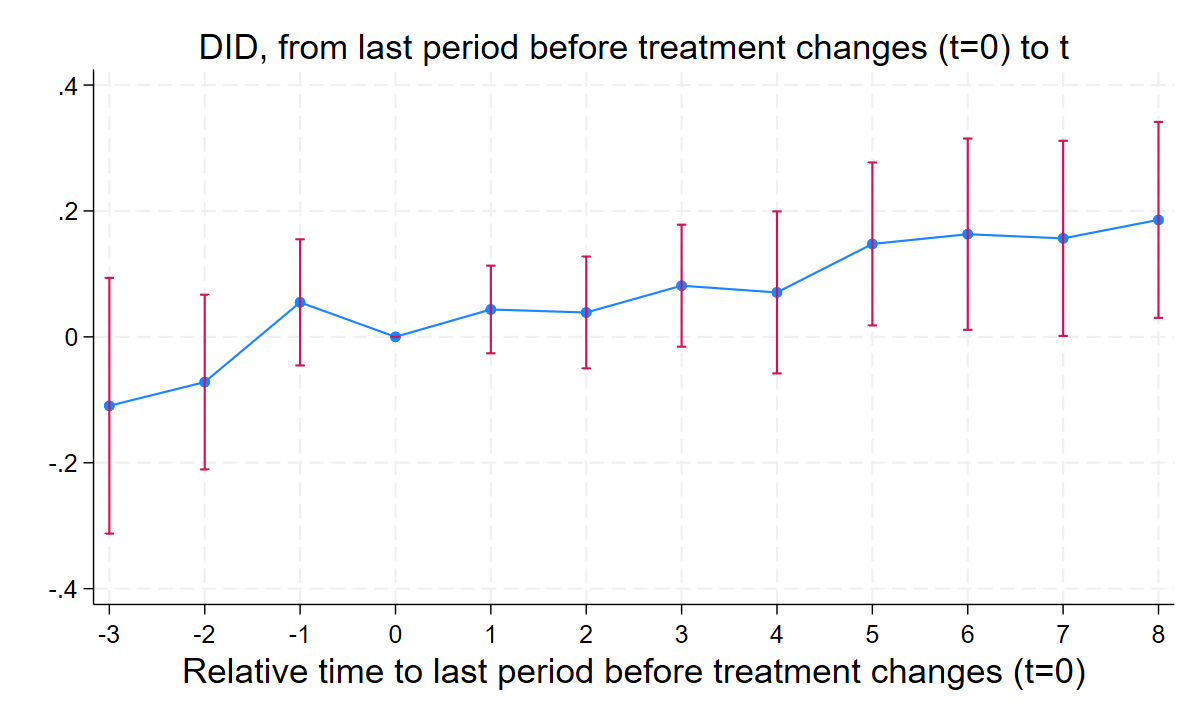
\includegraphics[width=0.9\linewidth]{figures/dch/favara_raw.png}
    \end{column}
  \end{columns}

  \smallskip
  \begin{readbox}
    \scriptsize
    In the eighth year counting the year of the first step, seven years after
    it, annual loan growth is $18.6$ log points above what it would have been
    had the county kept its initial index, for a county carrying $18.4$
    accumulated law-years on average.\\
    \textit{En el octavo año contando el del primer paso, siete años después, el
    crecimiento anual del crédito es 18.6 puntos logarítmicos mayor de lo que
    habría sido de haber mantenido el índice de partida, en un condado que
    acumula 18.4 ley-años de media.}
  \end{readbox}

\end{frame}

\begin{frame}{Case 1 --- From Raw to Normalized: Eight Effects Divided by the Dose}

  \footnotesize
  Two runs of the same command, without and with \texttt{normalized}. The
  command does not print $\delta^{D}_\ell$; dividing one run by the other
  recovers it, and consecutive differences approximate the extra laws in
  force at each horizon.

  \smallskip
  \begin{center}
  \begin{tabular}{@{}crrrrr@{}}
    \toprule
    $\ell$ & Raw $\text{DID}_\ell$ & Normalized $\text{DID}^{n}_\ell$ & Ratio $= \delta^{D}_\ell$, law-years & Difference & Switchers \\
    \midrule
    1 & 0.0435 & 0.0197 & 2.2  & 2.2 & 905 \\
    2 & 0.0387 & 0.0088 & 4.4  & 2.2 & 905 \\
    3 & 0.0813 & 0.0123 & 6.6  & 2.2 & 905 \\
    4 & 0.0706 & 0.0080 & 8.8  & 2.2 & 905 \\
    5 & 0.1476 & 0.0134 & 11.0 & 2.2 & 905 \\
    6 & 0.1631 & 0.0121 & 13.5 & 2.4 & 850 \\
    7 & 0.1565 & 0.0098 & 16.0 & 2.5 & 773 \\
    8 & 0.1858 & 0.0101 & 18.4 & 2.5 & 773 \\
    \bottomrule
  \end{tabular}
  \end{center}

  \smallskip
  The switcher mean rose by $2.2$ laws at its first change and kept them, so
  the accumulated column grows by $2.2$ a year while the switchers are the
  same $905$. The difference rises afterwards for two reasons, checked in the
  data: $101$ counties received further steps after their first change (the
  extra laws in force go $2.20, 2.19, 2.19, 2.20, 2.24, 2.28, 2.33, 2.47$),
  and from $\ell = 6$ the late switchers leave while the early ones had a
  slightly larger first change ($2.25$).

\end{frame}

\begin{frame}{Case 1 --- Normalized Effects: Per Law-Year}

  \begin{columns}[T]
    \begin{column}{0.46\textwidth}
      \footnotesize
      \texttt{... effects(8) placebo(3) cluster(state\_n) normalized
      normalized\_weights}

      \medskip
      \begin{readbox}
        \scriptsize
        At $\ell = 8$, each law-year received so far accounts for one log
        point of annual loan growth ($0.010$ in log units): one step adds
        about one point per year in force, flat across horizons.\\
        \textit{En el octavo año, cada ley-año recibido hasta entonces explica
        un punto logarítmico del crecimiento anual del crédito (0.010 en
        unidades log): un paso añade un punto
        por cada año en vigor, igual en todos los horizontes.}
      \end{readbox}

      \scriptsize Effects$_5$--$_8$ significant at 5\%; joint $p = 0.064$;
      placebos $p = 0.41$. The raw profile quadruples between $\ell = 1$ and
      $8$ while the exposure grows eightfold. Switchers fall from $\ell = 6$
      because the panel ends in 2005 (\texttt{same\_switchers} holds the sample
      fixed).
    \end{column}
    \begin{column}{0.54\textwidth}
      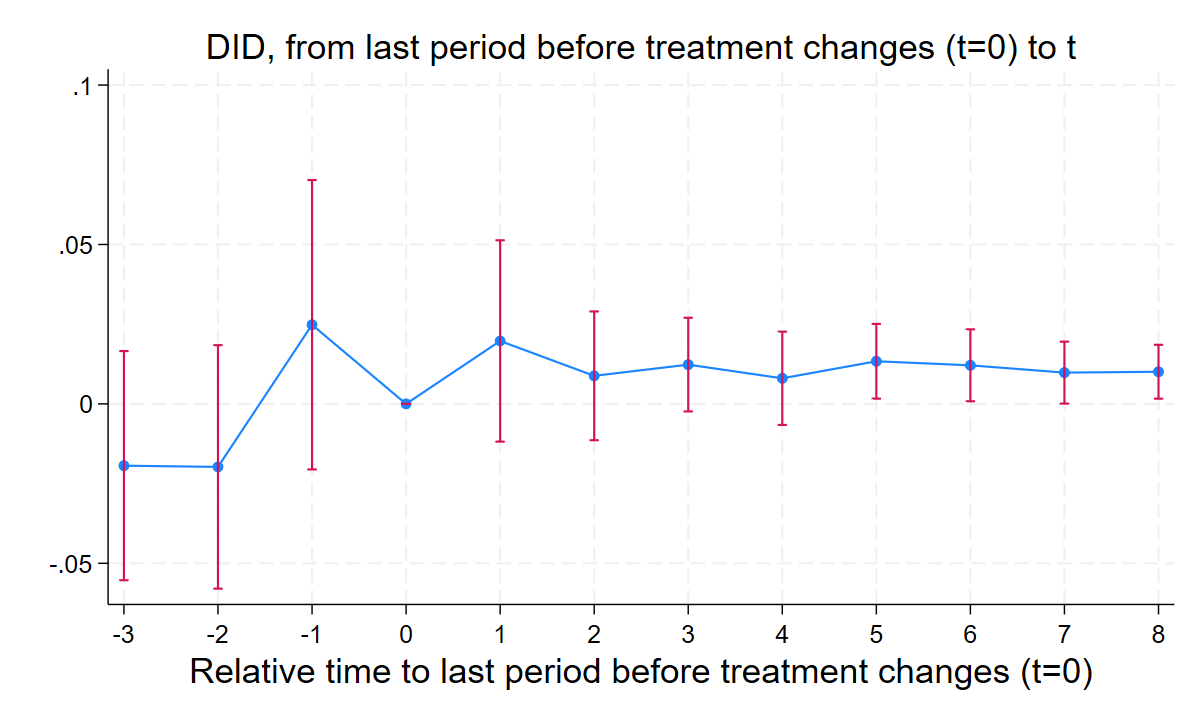
\includegraphics[width=\linewidth]{figures/dch/favara_normalized.png}
    \end{column}
  \end{columns}

\end{frame}

\begin{frame}{Case 1 --- \texttt{Av\_tot\_eff}, Step by Step}

  \footnotesize
  \begin{columns}[T]
    \begin{column}{0.52\textwidth}
      \begin{block}{\footnotesize Numerator: the raw effects, added over the window}
        \footnotesize
        $0.043 + 0.039 + 0.081 + 0.071 + 0.148 + 0.163 + 0.157 + 0.186 \approx 0.887$ (exact sum $0.8871$),
        unweighted; the command weights each horizon by its switchers.
      \end{block}

      \smallskip
      \begin{block}{\footnotesize Denominator: the extra laws in force, added over the window}
        \footnotesize
        $2.2 + 2.2 + 2.2 + 2.2 + 2.2 + 2.4 + 2.5 + 2.5 = 18.4$ law-years from
        the table.
      \end{block}

      \smallskip
      \[
        \hat\delta \approx \frac{0.887}{18.4} = 0.048
        \quad (\text{command, switcher-weighted: } 0.0478)
      \]
      One law-year raises loan growth by $4.8$ log points in total over the
      eight horizons.
    \end{column}
    \begin{column}{0.46\textwidth}
      \begin{block}{\footnotesize The output line ``average number of time periods over which a treatment's effect is accumulated $= 4.34$''}
        \footnotesize
        The paper's p.~10 quantity, computed from the dose paths, the last
        year each county has a same-baseline control and \texttt{effects(8)}: a law-year
        arriving at horizon $1$ of a county observed all eight horizons is
        counted $8$ times, one arriving at horizon $8$ once, and counties
        switching in 2000 or 2001 are observed fewer horizons before 2005.
        The dose-weighted average is $4.34$.
      \end{block}

      \smallskip
      \[
        \frac{0.048}{4.34} = 0.011 \approx \text{the flat normalized level}
      \]
      Per law-year and per year, $0.011$; counted over $4.34$ horizons on
      average, $0.048$. A shorter \texttt{effects()} lowers both the $4.34$
      and $\hat\delta$.
    \end{column}
  \end{columns}

\end{frame}

\begin{frame}{Case 1 --- \texttt{Av\_tot\_eff}: What It Says and What to Report}

  \begin{columns}[T]
    \begin{column}{0.50\textwidth}
      \begin{readbox}
        \scriptsize
        One deregulation step in force for one year raises annual loan growth
        by $4.8$ log points in total over the eight-year window, about $1.1$
        per year over the $4.3$ years it is counted.\\
        \textit{Un paso de desregulación en vigor un año eleva el crecimiento
        anual del crédito 4.8 puntos logarítmicos en total a lo largo de la
        ventana de ocho años, 1.1 por año durante los 4.3 años en que se
        cuenta.}
      \end{readbox}

      \smallskip
      \begin{block}{\footnotesize Which number is the headline}
        \footnotesize
        SE $0.025$, CI $[-0.001,\ 0.096]$, just including zero while four
        horizons are individually significant; identical with or without
        \texttt{normalized}. The normalized profile is flat, so $\hat\delta$
        summarizes it and the event study is the evidence that the design
        holds: placebos at $p = 0.41$, effects growing with the law-years and
        stable per law-year.
      \end{block}
    \end{column}
    \begin{column}{0.46\textwidth}
      \begin{block}{\footnotesize For your own design}
        \footnotesize
        Raw: outcome units at horizon $\ell$, actual path against status quo.
        Normalized: per dose-period accumulated up to $\ell$; recover the
        accumulated dose by dividing the two runs.
        \texttt{Av\_tot\_eff}: per dose-period, cumulated over your
        \texttt{effects()} window; set it against the cost of one dose-period,
        and report the window with it. Binary absorbing: normalized $=$
        raw$/\ell$ and \texttt{Av\_tot\_eff} $=$ the mean of the raw effects
        weighted by switchers per horizon.
      \end{block}
    \end{column}
  \end{columns}

\end{frame}

\begin{frame}{Case 1 --- \texttt{normalized\_weights}: Weights on Treatment Lags}

  \begin{columns}[T]
    \begin{column}{0.44\textwidth}
      \footnotesize
      A normalized Effect$_\ell$ blends the effect of the \emph{current} treatment
      ($k{=}0$) and its lags ($k{=}1,2,\dots$). The lags cannot be separated, but the
      \emph{weight} on each can be reported:

      \smallskip
      \scriptsize
      \begin{tabular}{@{}crrrr@{}}
        \toprule
        $k$ & $\ell{=}1$ & $\ell{=}2$ & $\ell{=}4$ & $\ell{=}8$ \\
        \midrule
        0 & \textbf{1.00} & 0.50 & 0.25 & 0.13 \\
        1 & ---  & 0.50 & 0.25 & 0.13 \\
        2 & ---  & ---  & 0.25 & 0.13 \\
        3 & ---  & ---  & 0.25 & 0.12 \\
        $\vdots$ &   &   &   & $\vdots$ \\
        7 & ---  & ---  & ---  & 0.12 \\
        \midrule
        Tot. & 1.00 & 1.00 & 1.00 & 1.00 \\
        \bottomrule
      \end{tabular}
    \end{column}
    \begin{column}{0.52\textwidth}
      \begin{block}{How to read it}
        \footnotesize
        \begin{itemize}\footnotesize
          \item Effect$_1$: all weight on $k{=}0$: only the current dose, no lags yet.
          \item Effect$_2$: half on the current dose, half on the 1-period lag.
          \item Effect$_8$: $\approx 0.12$--$0.13$ on \emph{each} of $k{=}0,\dots,7$
            , nearly uniform.
        \end{itemize}
      \end{block}

      \smallskip
      \footnotesize
      Each weight is the share of the law-years received so far that comes from
      that lag: $\approx 1/8$ each at $\ell=8$ because a law, once passed,
      stays. So
      Effect$_8$ is the average contribution of a law-year over eight years of
      exposure, not the effect of a law eight years after it passed.

      \smallskip
      \textbf{Applied conclusion:} Favara's pair (raw rising with the
      law-years, normalized flat) is the persistent case of the worked example.
      Whether one step fades or builds needs \texttt{by\_path} or
      \texttt{normalized effects\_equal}.
    \end{column}
  \end{columns}

\end{frame}

% ════════════════════════════════════════════════════════════════════════
% CASE 4: GENTZKOW ET AL. (2011) — Textbook pre-trends
% ════════════════════════════════════════════════════════════════════════

\begin{frame}{Case 4 --- Gentzkow et al.\ (2011): Context \& Data}

  \begin{columns}[T]
    \begin{column}{0.50\textwidth}
      \textbf{Research question}\\
      Do local daily newspapers affect voter turnout?

      \medskip
      \textbf{Paper}\\
      Gentzkow, Shapiro \& Sinkinson (2011),
      \textit{AER} 101(7): 2980--3018.

      \medskip
      \textbf{Data} (replication package)\\
      Unbalanced panel of \textbf{1{,}195 US counties}
      $\times$ \textbf{16 presidential-election years} (1868--1928);
      16{,}872 obs.\\[3pt]
      Outcome \texttt{prestout} (turnout rate); treatment
      \texttt{numdailies} (number of daily papers).
    \end{column}
    \begin{column}{0.46\textwidth}
      \begin{block}{Design (read off the data)}
        \footnotesize
        \begin{itemize}\footnotesize
          \item Baseline treatment is \textbf{multivalued}
            (0 to 33; 75.6\% of counties start at 0).
          \item Counties \textbf{gain and lose} papers
            ($\Delta$ both $+$ and $-$).
          \item \textbf{81\%} of counties change their count
            \textbf{two or more times}.
        \end{itemize}
      \end{block}

      \smallskip
      \footnotesize A multivalued, non-absorbing treatment: no single
      first-treatment date, so identify from each change and normalize
      by switch size.
    \end{column}
  \end{columns}

\end{frame}

\begin{frame}[fragile]{Case 4 --- Effects Significant, Pre-Trends Flat}

  \begin{columns}[T]
    \begin{column}{0.44\textwidth}
\begin{lstlisting}
did_multiplegt_dyn      ///
  prestout              ///
  cnty90 year           ///
  numdailies,           ///
  effects(4) placebo(4) ///
  cluster(cnty90)       ///
  effects_equal("all")
\end{lstlisting}

      \smallskip\footnotesize
      \textbf{Results:}
      \begin{itemize}
        \item Effects: 0.014, 0.019, 0.021, 0.027; joint $p = 0.007$
        \item effects\_equal $p = 0.415$ (stable over time)
        \item Placebos: $-0.001$, $0.002$, $-0.002$, $0.001$;
          \textbf{placebo $p = 0.992$} \checkmark\checkmark\checkmark
      \end{itemize}
    \end{column}
    \begin{column}{0.54\textwidth}
      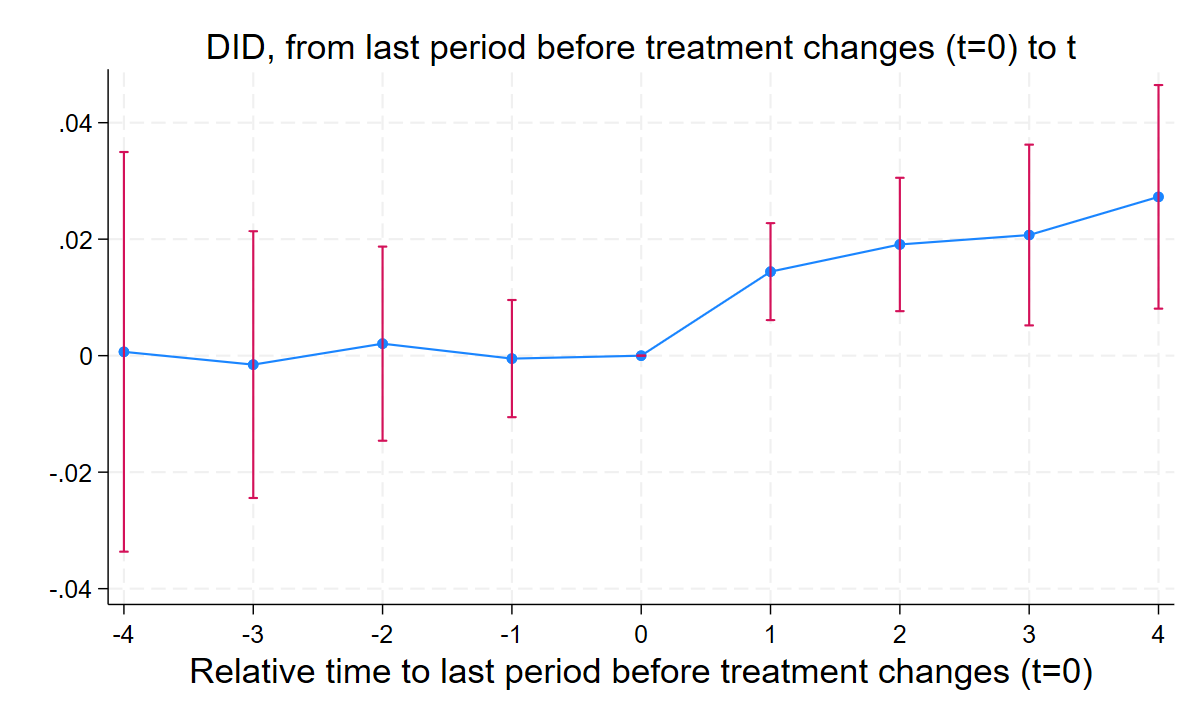
\includegraphics[width=0.9\linewidth]{figures/dch/gentzkow_effects.png}
    \end{column}
  \end{columns}

  \smallskip
  \begin{readbox}
    \scriptsize
    In the election in which the number of dailies changes, by $1.2$ on
    average, turnout is $1.4$ points higher than it would have been with the
    previous count, on a $65$\,\% base; $2.7$ points by the fourth election,
    three elections later.\\
    \textit{En la elección en que cambia el número de diarios (1.2 de media),
    la participación es 1.4 puntos mayor de lo que habría sido con el número
    anterior, sobre una base del 65\,\%; 2.7 puntos en la cuarta elección,
    tres después.}
  \end{readbox}

\end{frame}

\begin{frame}[fragile]{Case 4 --- Normalized: Effect per Newspaper-Election}

  \begin{columns}[T]
    \begin{column}{0.44\textwidth}
\begin{lstlisting}
did_multiplegt_dyn      ///
  prestout cnty90       ///
  year numdailies,      ///
  effects(4) placebo(4) ///
  cluster(cnty90)       ///
  normalized            ///
  normalized_weights    ///
  effects_equal("all")
\end{lstlisting}

      \smallskip\footnotesize
      \textbf{Per newspaper-election:} effects 0.012, 0.008, 0.006, 0.005;
      placebo $p = 0.992$; \texttt{Av\_tot\_eff} $= 0.016$.

      \smallskip
      \scriptsize The decline is not significant ($p = 0.165$). It suggests
      lagged papers matter less than current ones (companion, pp.~39--40); a
      direct test that the first lag has no effect gives $p = 0.83$ (p.~40).
    \end{column}
    \begin{column}{0.54\textwidth}
      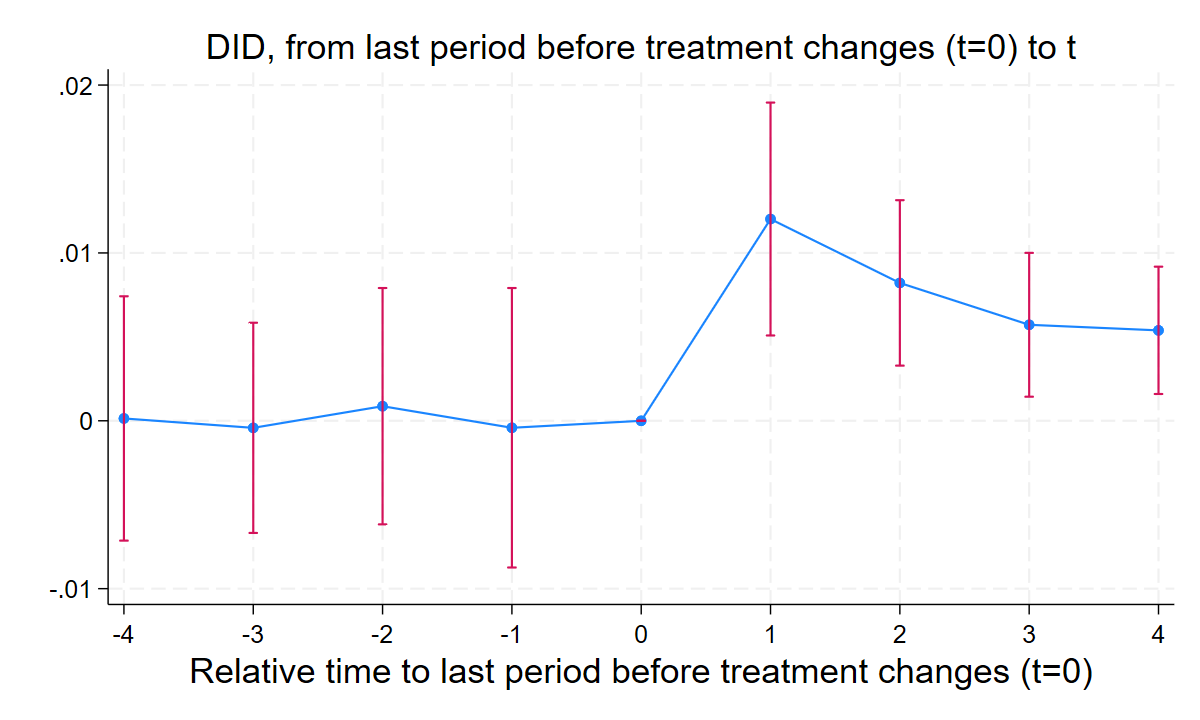
\includegraphics[width=0.9\linewidth]{figures/dch/gentzkow_normalized.png}
    \end{column}
  \end{columns}

  \smallskip
  \begin{readbox}
    \scriptsize
    Per newspaper-election, turnout is $1.2$ points higher in the election of
    the change and $0.5$ by the fourth, three elections later; one newspaper in
    circulation for one election raises turnout $1.6$ points in total over the
    four-election window.\\
    \textit{Por periódico-elección, la participación sube 1.2 puntos en la
    elección del cambio y 0.5 en la cuarta, tres después; un periódico en
    circulación durante una elección sube la participación 1.6 puntos en total
    en la ventana de cuatro elecciones.}
  \end{readbox}

\end{frame}

\begin{frame}[fragile]{Case 4 --- Treatment Paths and Composition}

  \begin{columns}[T]
    \begin{column}{0.50\textwidth}
      \textbf{Which paths identify the effect?} (\texttt{design})
      \begin{itemize}\footnotesize
        \item The estimate pools \emph{many} distinct treatment paths.
        \item Most common: $0\to(1,1,1,1)$, 15\% of the 933 switchers
          observed four elections; next, enter-then-exit, 14\%.
        \item The listed paths cover 80\% of them.
      \end{itemize}

      \smallskip
      \footnotesize Transparency about \emph{what variation} drives the
      estimate, like \texttt{normalized\_weights} earlier.
    \end{column}
    \begin{column}{0.46\textwidth}
      \begin{block}{Composition (\texttt{same\_switchers})}
        \footnotesize
        Holding the sample fixed at the \textbf{907 switchers} present at
        every horizon: effects $0.013\to0.029$ (joint $p=0.019$), placebo
        $p=0.93$.\\[4pt]
        Close to the baseline, so the growing event study is \textbf{not}
        a composition artefact.
      \end{block}
    \end{column}
  \end{columns}

\end{frame}

% ── Practical card: running dCH ──────────────────────────────────────────
\begin{frame}{Running dCH --- The Practical Answers}

  \begin{columns}[T]
    \begin{column}{0.48\textwidth}
      \textbf{At what level do I cluster?}\\
      \footnotesize At $g$ or coarser, never finer: with $g$ = county and a
      state policy, \texttt{cluster(state)}; with $g$ = state, a state weighs
      its number of counties.

      \medskip
      \normalsize\textbf{How many effects and placebos?}\\
      \footnotesize \texttt{placebo()} must not exceed \texttt{effects()}. The
      horizon is capped by the data at $\ell_{\max} = T_g - F_g + 1$, and the
      switcher count falls as $\ell$ grows. Read that column before you read the
      coefficients.

      \medskip
      \normalsize\textbf{\texttt{normalized} or not?}\\
      \footnotesize If the dose varies in size, yes: without it a
      $0\!\to\!1$ and a $0\!\to\!4$ switch are averaged as the same event. The
      normalized effect averages over doses \emph{and} lags, with the lag
      weights printed by \texttt{normalized\_weights}. When a few paths
      dominate, \texttt{by\_path()} gives each path's effect against the status
      quo with no normalization; the price is switchers per path.
    \end{column}
    \begin{column}{0.48\textwidth}
      \begin{block}{\footnotesize Which number goes in the report?}
        \footnotesize
        Raw Effect$_\ell$: outcome units at horizon $\ell$, actual path against
        status quo. Normalized: per dose-period accumulated up to $\ell$.
        \texttt{Av\_tot\_eff}: per dose-period, cumulated over the
        \texttt{effects()} window, the cost-benefit number (p.~9). The event
        study is the \emph{evidence} that the design holds. Course rule: the
        headline is \texttt{Av\_tot\_eff} when the normalized profile is
        stable, the per-horizon effects when it is not.
      \end{block}

      \smallskip
      \begin{alertblock}{\footnotesize Two things that are not errors}
        \footnotesize
        Wide confidence intervals when few units switch, and effects that stop
        at a short horizon because the panel ends. Both are the estimator
        reporting the precision your data actually support.
      \end{alertblock}

      \smallskip
      \footnotesize Placebos that fail, sequential treatments and continuous
      doses come next.
    \end{column}
  \end{columns}

\end{frame}

\recapdch

% ════════════════════════════════════════════════════════════════════════
% CASE 2: DERYUGINA (2017) — Parallel trends fail
% ════════════════════════════════════════════════════════════════════════

\begin{frame}{Case 2 --- Deryugina (2017): Context \& Data}

  \begin{columns}[T]
    \begin{column}{0.50\textwidth}
      \textbf{Research question}\\
      How do hurricanes affect non-disaster government transfers to
      counties?

      \medskip
      \textbf{Paper}\\
      Deryugina (2017), \textit{AEJ: Policy} 9(3): 168--198.

      \medskip
      \textbf{Data} (replication package)\\
      Unbalanced panel of \textbf{1{,}183 US counties}
      $\times$ \textbf{44 years} (1969--2012); 49{,}698 obs.\\[3pt]
      Outcome \texttt{log\_curr\_trans\_ind\_gov\_pc} (log non-disaster
      transfers p.c.); treatment \texttt{hurricane} (0/1).
    \end{column}
    \begin{column}{0.46\textwidth}
      \begin{block}{Design (read off the data)}
        \footnotesize
        \begin{itemize}\footnotesize
          \item Binary, \textbf{non-absorbing}: each county's total
            hurricane count is \textbf{0 or 1}: hit in at most one
            year (on, then off).
          \item \textbf{361} of 1{,}183 counties are ever hit.
        \end{itemize}
      \end{block}

      \smallskip
      \begin{alertblock}{\footnotesize The cautionary tale}
        \footnotesize
        Before the hurricane, transfers in hit counties were already
        \emph{rising} relative to unhit counties (all six placebos negative),
        so the placebos fail and the effects are likely overstated. dCH
        \emph{diagnoses} the violation; it does not fix it.
      \end{alertblock}
    \end{column}
  \end{columns}

\end{frame}

\begin{frame}{Case 2 --- First Estimates: Large, Growing, Significant}

  \begin{columns}[T]
    \begin{column}{0.44\textwidth}
      \footnotesize
      \textbf{Effect of a hurricane} (no controls):

      \smallskip
      \begin{tabular}{@{}ccc@{}}
        \toprule
        $\ell$ & Effect & sig.? \\
        \midrule
        1 & 0.011 & \checkmark \\
        2 & 0.013 & \checkmark \\
        3 & 0.016 & \checkmark \\
        4 & 0.016 & \checkmark \\
        5 & 0.023 & \checkmark \\
        6 & 0.027 & \checkmark \\
        \bottomrule
      \end{tabular}

      \smallskip
      Joint $p = 8\times10^{-13}$; \textbf{Av\_tot\_eff} $= 0.106$.
    \end{column}
    \begin{column}{0.52\textwidth}
      \begin{block}{\footnotesize A transient shock, a persistent effect}
        \footnotesize
        \texttt{hurricane} is $1$ for a single year, then $0$. Transfers stay
        elevated and keep rising up to five years later; the dynamic estimator traces
        the carryover, which a method assuming the effect lasts only while
        $D = 1$ would miss.
      \end{block}

      \smallskip
      \begin{alertblock}{\footnotesize But can we believe it?}
        \footnotesize
        Positive, growing, hugely significant. The question first: do the
        pre-treatment placebos hold?
      \end{alertblock}
    \end{column}
  \end{columns}

  \smallskip
  \begin{readbox}
    \scriptsize
    Transfers per capita are $1.1$\,\% higher in the hurricane year than they
    would have been without it, and $2.7$\,\% five years later; a hurricane
    raises transfers by $10.6$\,\% of one year's transfers in total over six
    years.\\
    \textit{Las transferencias per cápita son un 1.1\,\% mayores el año del
    huracán de lo que habrían sido sin él, y un 2.7\,\% cinco años después; un
    huracán eleva las transferencias un 10.6\,\% de las de un año en total a lo
    largo de seis años.}
  \end{readbox}

\end{frame}

\begin{frame}[fragile]{Case 2 --- Pre-Trends That Fail (and Partially Improve)}

  \begin{columns}[T]
    \begin{column}{0.54\textwidth}
      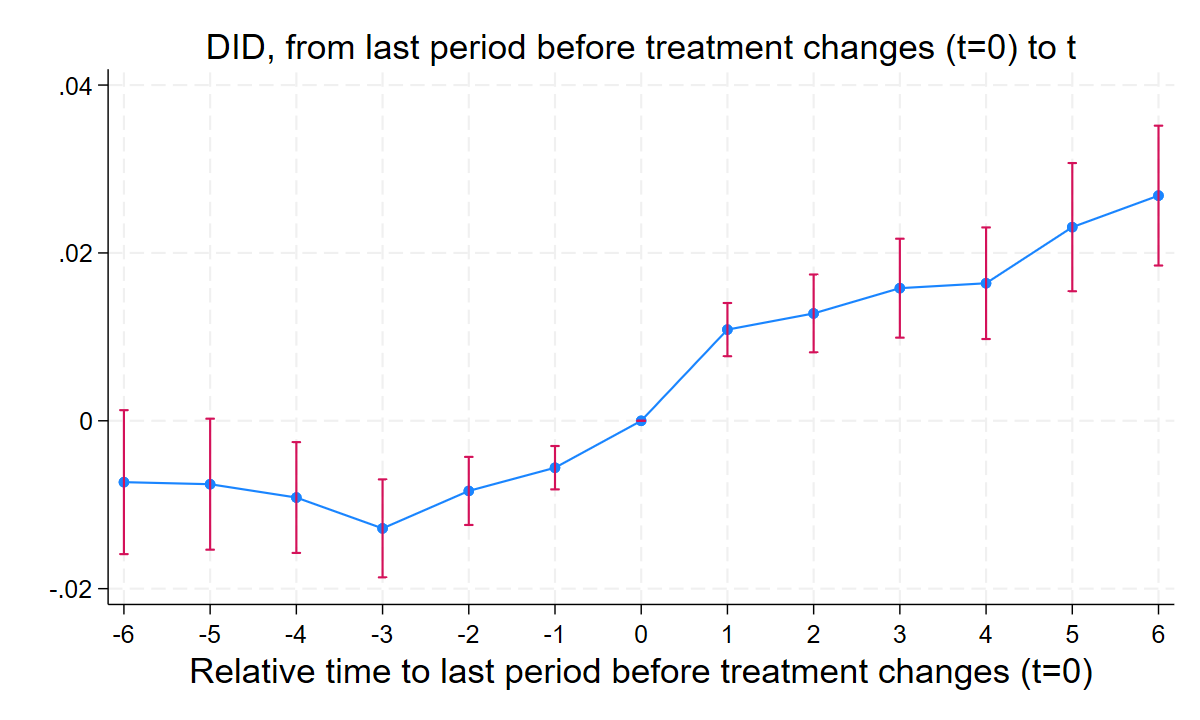
\includegraphics[width=0.49\linewidth]{figures/dch/deryugina_nocontrols.png}%
      \hfill%
      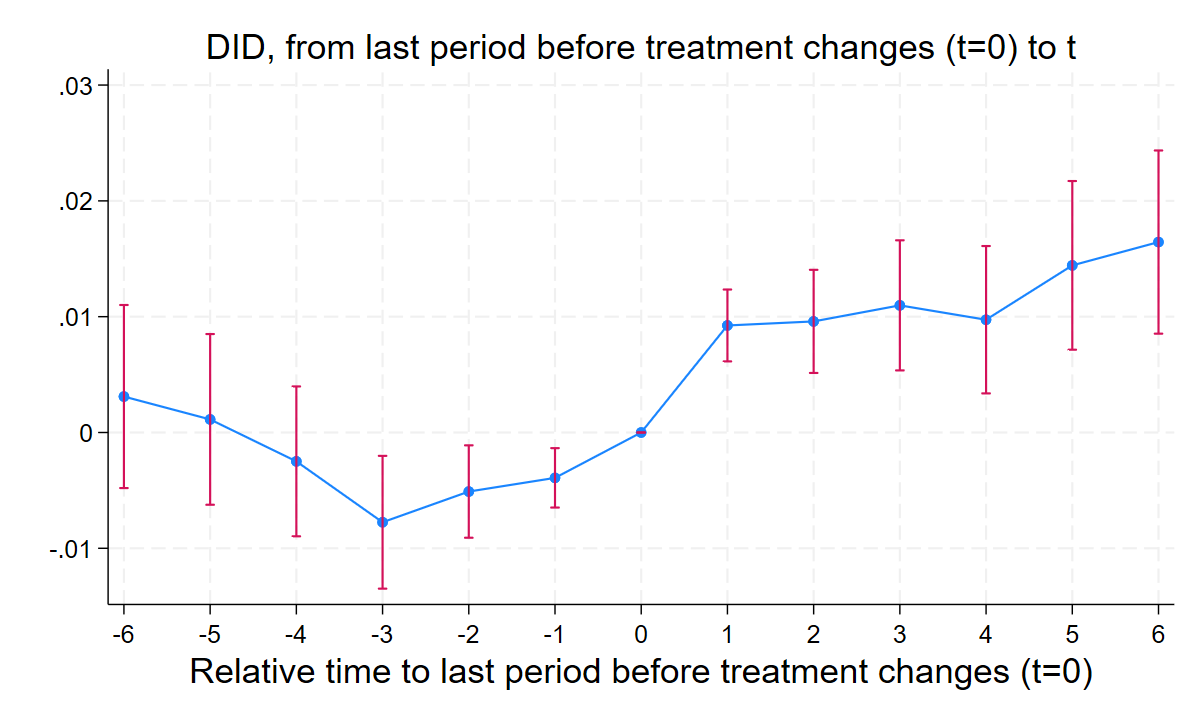
\includegraphics[width=0.49\linewidth]{figures/dch/deryugina_controls.png}

      \smallskip\centering\footnotesize
      Left: no controls \hfill Right: with pre-trend controls
    \end{column}
    \begin{column}{0.44\textwidth}
\begin{lstlisting}
* Without controls:
did_multiplegt_dyn      ///
  log_curr_trans_ind_gov_pc ///
  county_fips year      ///
  hurricane,            ///
  effects(6) placebo(6) ///
  cluster(county_fips)

* With baseline char. x year:
did_multiplegt_dyn ..., ///
  effects(6) placebo(6) ///
  controls(`controls')  ///
  cluster(county_fips)
\end{lstlisting}

      \smallskip\footnotesize
      \textbf{Without controls:}\\
      Placebo $p = 4.3\!\times\!10^{-6}$ \alert{$\times$}

      \smallskip
      \textbf{With controls:}\\
      Placebo $p = 0.000035$ \alert{$\times$}

      \smallskip
      \textbf{Lesson:} controls improve but do
      not resolve the violation. The problem
      is fundamental. Report it.
    \end{column}
  \end{columns}

\end{frame}

\begin{frame}{Case 2 --- When Parallel Trends Fail: What To Do}

  \begin{columns}[T]
    \begin{column}{0.50\textwidth}
      \textbf{Option 1: Add controls (char.\ $\times$ year)}
      \begin{itemize}\small
        \item Allow each type of unit to follow
          its own linear trend
        \item Deryugina: $p$ goes from $4.3\!\times\!10^{-6}$
          to $3.5\!\times\!10^{-5}$, still fails
        \item Only works when the trend difference
          is proportional to observables
      \end{itemize}

      \medskip
      \textbf{Option 2: \texttt{trends\_nonparam}}
      \begin{itemize}\small
        \item Year effects by a time-invariant set
          coarser than the unit (e.g.\ state)
        \item For states or industries on different trends
      \end{itemize}

      \medskip
      \textbf{Option 3: Restrict sample}
      \begin{itemize}\small
        \item Compare only geographically or
          demographically similar units
      \end{itemize}
    \end{column}
    \begin{column}{0.46\textwidth}
      \textbf{Option 4: Report as limitation}
      \begin{itemize}\small
        \item Pre-trend failure is informative
          : it shows \emph{which} units drive
          the violation
        \item Reporting the PT failure is
          preferable to ignoring it
      \end{itemize}

      \medskip
      \begin{alertblock}{\footnotesize Key takeaway}
        \footnotesize dCH \emph{diagnoses} the
        problem. It does not guarantee
        a fix. That requires subject-matter
        knowledge and, often, a better design.\\[4pt]
        Reporting the failure is preferable to
        leaving it undetected.
      \end{alertblock}
    \end{column}
  \end{columns}

\end{frame}

\begin{frame}{Cases 2 vs.\ 4 --- Same Estimator, Different Pre-Trends}

  \textbf{Same command, same country, opposite pre-trend results.}

  \bigskip
  \begin{columns}[T]
    \begin{column}{0.48\textwidth}
      \begin{alertblock}{\textbf{Deryugina (2017)}: \alert{Fails}}
        Placebo joint $p = 4.3\!\times\!10^{-6}$\\[4pt]
        All placebos are negative: before the
        hurricane, hit counties' transfers were
        already \emph{rising} relative to unhit
        counties, so the effect is likely overstated.\\[4pt]
        Adding controls does not resolve it.
      \end{alertblock}
    \end{column}
    \begin{column}{0.48\textwidth}
      \begin{exampleblock}{\textbf{Gentzkow et al.\ (2011)}: \checkmark\ Passes}
        Placebo joint $p = 0.992$\\[4pt]
        No evidence that counties changing their
        newspaper count trended differently from
        stable counties in prior elections.\\[4pt]
        This supports parallel trends but does not
        prove it: the test can lack power (Roth 2022).
      \end{exampleblock}
    \end{column}
  \end{columns}

  \smallskip
  \centering\small
  The pre-trend test reflects whether the design is credible;
  the result depends on the data, not on the researcher's choice.

  \smallskip
  \raggedright\footnotesize
  \textbf{When a placebo rejects, its sign suggests the bias direction}, if
  the pre-switch trend gap continues after the switch: placebos run backward
  from $F_g-1$ (p.~11), so a negative placebo suggests an upward bias.

\end{frame}

% ════════════════════════════════════════════════════════════════════════
% CASE 5: HOLLINGSWORTH ET AL. (2022) — Sequential binary treatment
% ════════════════════════════════════════════════════════════════════════

\begin{frame}{Case 5 --- Hollingsworth et al.\ (2022): Context \& Data}

  \begin{columns}[T]
    \begin{column}{0.50\textwidth}
      \textbf{Research question}\\
      How do medical (mm) and recreational (rm) marijuana laws affect
      marijuana use?

      \medskip
      \textbf{Paper}\\
      Hollingsworth, Wing \& Bradford (2022),
      \textit{J.\ Law and Economics} 65(3): 515--554.

      \medskip
      \textbf{Data} (replication package)\\
      \textbf{51 states} $\times$ \textbf{15 years} (2002--2016); 765 obs.\\[3pt]
      Outcome \texttt{ln\_mj\_use\_365} (log past-year use); treatments
      \texttt{mm} and \texttt{rm} (both 0/1).
    \end{column}
    \begin{column}{0.46\textwidth}
      \begin{block}{Design (read off the data)}
        \footnotesize
        \begin{itemize}\footnotesize
          \item \textbf{Two sequential binary} treatments, both
            \textbf{absorbing} (no reversals); \texttt{rm} only after
            \texttt{mm}.
          \item \textbf{29} states adopt mm; only \textbf{7} adopt rm.
        \end{itemize}
      \end{block}

      \smallskip
      \footnotesize Estimate each separately: mm on states without rm; rm
      on states with mm, with \texttt{trends\_nonparam(fg1)} (trends by
      mm-adoption cohort). The few switchers foreshadow wide CIs.
    \end{column}
  \end{columns}

\end{frame}

\begin{frame}[fragile]{Case 5 --- Medical and Recreational Marijuana}

  \begin{columns}[T]
    \begin{column}{0.42\textwidth}
\begin{lstlisting}
* Effect of mm (rm==0 states):
did_multiplegt_dyn      ///
  ln_mj_use_365 state   ///
  year mm if rm==0,     ///
  effects(3) placebo(3) ///
  cluster(state)

* Effect of rm (mm==1 states):
did_multiplegt_dyn      ///
  ln_mj_use_365 state   ///
  year rm if mm==1,     ///
  effects(3) placebo(3) ///
  trends_nonparam(fg1)  ///
  cluster(state)
\end{lstlisting}
    \end{column}
    \begin{column}{0.56\textwidth}
      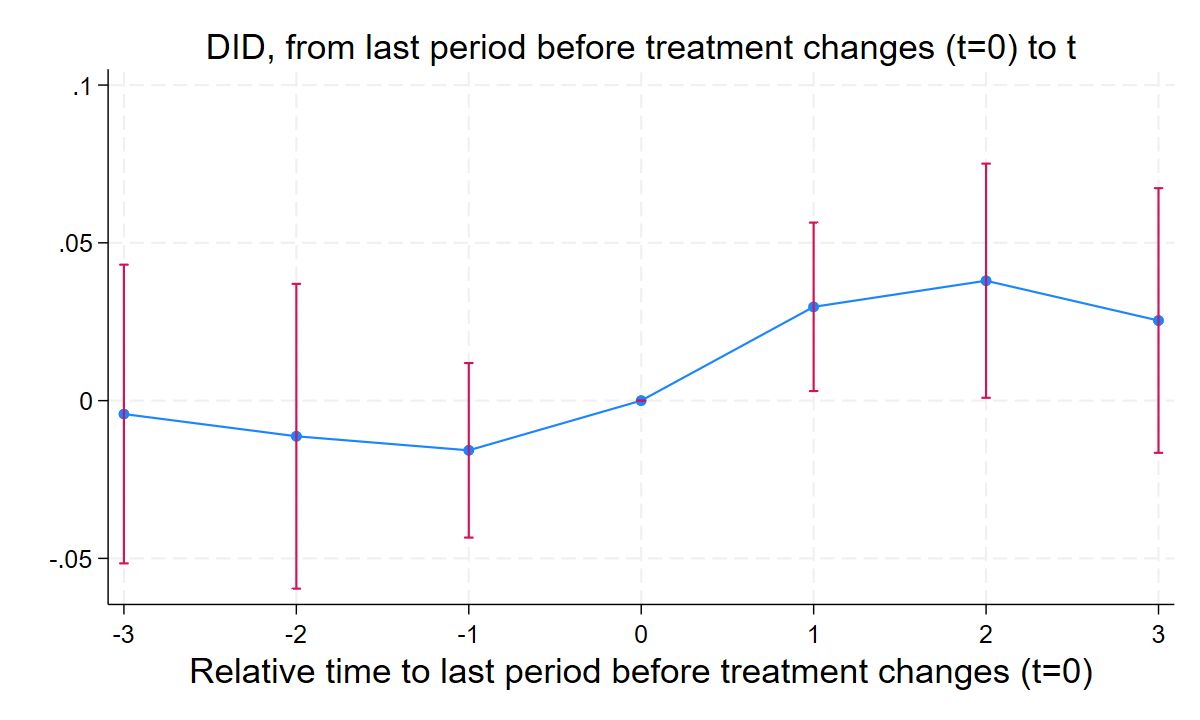
\includegraphics[width=0.49\linewidth]{figures/dch/hollingsworth_mm.png}%
      \hfill%
      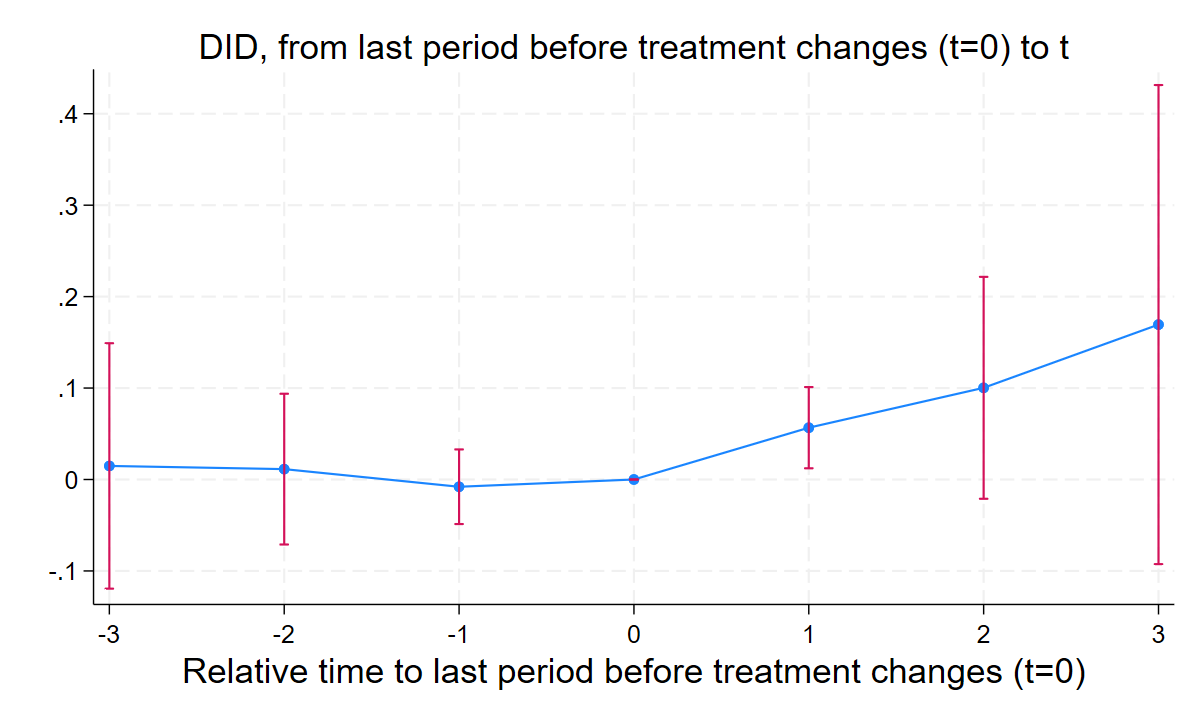
\includegraphics[width=0.49\linewidth]{figures/dch/hollingsworth_rm.png}

      \centering\scriptsize
      Left: medical marijuana \hfill Right: recreational

      \smallskip\raggedright\footnotesize
      \textbf{mm} (21 switchers): effects $0.030$, $0.038$, $0.025$, $p = 0.155$;
      placebo $p = 0.711$ \checkmark\\[2pt]
      \textbf{rm} (7 switchers!): effects $0.057$--$0.169$, $p = 0.066$;
      placebo $p = 0.933$ \checkmark\\[2pt]
      Wide CIs $=$ few states, not zero effect.
    \end{column}
  \end{columns}

  \smallskip
  \begin{readbox}
    \scriptsize
    Past-year use is $3.0$\,\% higher in the first year of a medical law than
    it would have been without one; one year of the law in force raises use
    $3.1$\,\% in total over the three-horizon window; $21$ switchers in year
    one, $16$ in year three.\\
    \textit{El consumo en el último año es un 3.0\,\% mayor el primer año de la
    ley medicinal de lo que habría sido sin ley; un año de ley en vigor eleva
    el consumo un 3.1\,\% en total en la ventana de tres horizontes; 21
    switchers en el año uno, 16 en el tres.}
  \end{readbox}

\end{frame}

\begin{frame}{Case 5 --- Why \texttt{trends\_nonparam(fg1)} for the rm Estimation}

  \textbf{Problem:} mm=1 states differ in years of mm exposure, so a change
  in ln\_mj\_use around rm adoption can come from one more year of mm.

  \medskip
  \begin{columns}[T]
    \begin{column}{0.50\textwidth}
      \textbf{The identification concern:}
      \begin{itemize}\small
        \item If the mm effect varies with exposure, states
          with different mm dates diverge even without rm
        \item fg1 compares rm adopters only with
          non-adopters that passed mm the same year
        \item Assumes one more year of mm has the
          same effect in every state
      \end{itemize}
    \end{column}
    \begin{column}{0.46\textwidth}
      \begin{block}{\texttt{trends\_nonparam(fg1)}}
        \footnotesize
        \textbf{fg1} = year of first mm adoption.\\[4pt]
        Each mm cohort follows its own
        non-parametric time trend.
        Units are compared only to other
        units within the same mm cohort.\\[4pt]
        More flexible than a linear trend
        control; fully non-parametric within
        cohort. Accounts for the sequential
        structure of the design.
      \end{block}
    \end{column}
  \end{columns}

  \smallskip
  \footnotesize \textbf{What you are buying:} parallel trends (assumption~2)
  need hold only among states with the same baseline dose \emph{and} mm
  cohort (companion, assumption~5, p.~20); a switcher with no
  not-yet-switcher in its cohort is dropped.

\end{frame}

\begin{frame}{Case 5 --- The Precision Cost of Clean Identification}

  \begin{columns}[T]
    \begin{column}{0.52\textwidth}
      \textbf{Why are CIs so wide for rm?}
      \begin{itemize}\small
        \item dCH uses only \emph{active switchers}
          for identification
        \item For rm: only 7 states switch
          $0\!\to\!1$ during 2002--2016, and the
          count falls with the horizon:
          \textbf{7 states at $\ell=1$, 5 at
          $\ell=2$, 2 at $\ell=3$}
        \item Small effective N $\Rightarrow$
          large standard errors
        \item Joint $p = 0.066$; only Effect$_1$ is
          significant at 5\%, Effects$_2$ and $_3$ are not
      \end{itemize}

      \smallskip
      \textbf{What TWFE does instead:}\\
      Uses all mm=1 states, including earlier
      rm adopters, as controls: smaller SEs, but
      centred on a coefficient biased by
      heterogeneous effects.
    \end{column}
    \begin{column}{0.44\textwidth}
      \begin{alertblock}{Precision reflects the data}
        \footnotesize
        dCH identifies only from genuine
        variation, so it reports the precision
        the data actually support.\\[4pt]
        Wide CIs here mean too few switchers to
        be precise, not a zero effect.\\[4pt]
        Report the CIs; do not read wide
        intervals as ``no effect.''
      \end{alertblock}
    \end{column}
  \end{columns}

\end{frame}

% ════════════════════════════════════════════════════════════════════════
% CASE 3: EAST ET AL. (2023) — Continuous treatment
% ════════════════════════════════════════════════════════════════════════

\begin{frame}{Case 3 --- East et al.\ (2023): Context \& Data}

  \begin{columns}[T]
    \begin{column}{0.50\textwidth}
      \textbf{Research question}\\
      Does prenatal Medicaid eligibility improve infant health (birth
      weight)?

      \medskip
      \textbf{Paper}\\
      East, Miller, Page \& Wherry (2023), \textit{AER} 113(1): 98--135.

      \medskip
      \textbf{Data} (replication package)\\
      \textbf{50 states} $\times$ \textbf{14 birth cohorts} (1975--1988);
      700 obs.\\[3pt]
      Outcome \texttt{lbw\_detrend81} (\% low birth weight, detrended to
      1981); treatment \texttt{newsimeli} (Medicaid eligibility rate).
    \end{column}
    \begin{column}{0.46\textwidth}
      \begin{block}{Design (read off the data)}
        \footnotesize
        \begin{itemize}\footnotesize
          \item \textbf{Continuous} treatment: 78 distinct values,
            range $0.04$--$0.28$.
          \item \textbf{Absorbing}: eligibility only rises (28 increases,
            0 decreases).
          \item \textbf{28} switchers.
        \end{itemize}
      \end{block}

      \smallskip
      \footnotesize Use \texttt{continuous(1)}. The raw \texttt{Effect\_}$\ell$
      is then the \textbf{level} effect of having expanded eligibility (the
      numerator uses a binarised switch indicator); \texttt{Av\_tot\_eff} and
      \texttt{normalized} divide by the actual change in \texttt{newsimeli}
      and are \textbf{per unit of eligibility} (companion, pp.~22--23): a
      scaled level, not a derivative.
    \end{column}
  \end{columns}

\end{frame}

\begin{frame}[fragile]{Case 3 --- Continuous Treatment Results}

  \begin{columns}[T]
    \begin{column}{0.44\textwidth}
\begin{lstlisting}
* $stcontrols: state x year
*   demographics (see do-file)
did_multiplegt_dyn lbw_detrend81       ///
  plborn dob_y_p newsimeli,            ///
  effects(5) placebo(5) continuous(1)  ///
  controls($stcontrols) weight(births) ///
  effects_equal("all")
\end{lstlisting}

      \smallskip\footnotesize
      \textbf{Results:}
      \begin{itemize}
        \item Effects: $-0.095 \to -0.287$ (negative and growing);
          joint $p = 0.014$ \checkmark
        \item effects\_equal $p = 0.186$ (stable); placebo $p = 0.721$ \checkmark
        \item 28 switchers
      \end{itemize}

    \end{column}
    \begin{column}{0.54\textwidth}
      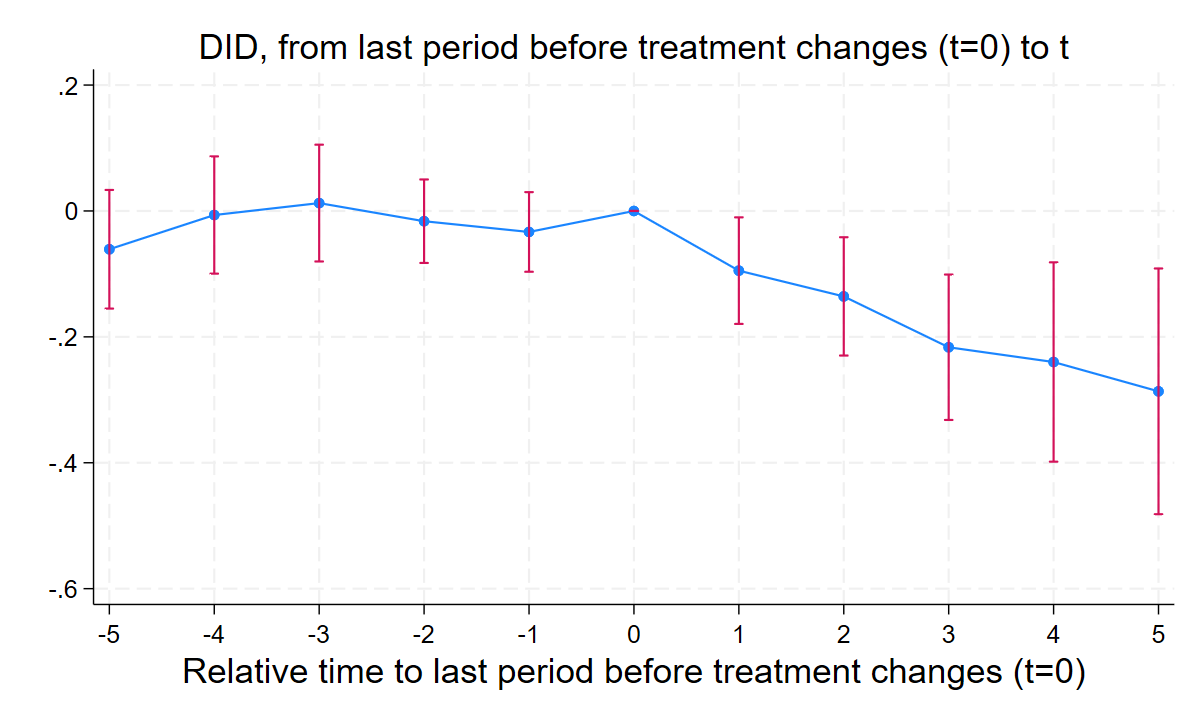
\includegraphics[width=0.78\linewidth]{figures/dch/east_continuous.png}

      {\scriptsize\itshape SEs shown are analytic; with \texttt{continuous()}
      dCH recommend \texttt{bootstrap}.}
    \end{column}
  \end{columns}

  \smallskip
  \begin{readbox}
    \scriptsize
    The low-birth-weight rate is $0.09$ points lower in the year of an
    expansion, of $7.3$ points of eligibility on average, and $0.29$ points
    lower in the fifth year, four years later; per unit of eligibility (100
    points) in force for one year, $2.67$ points lower in total
    (\texttt{Av\_tot\_eff}), that is $0.27$ per 10 points.\\
    \textit{La tasa de bajo peso es 0.09 puntos menor el año de una expansión,
    de 7.3 puntos de elegibilidad de media, y 0.29 puntos menor en el quinto
    año, cuatro después; por unidad de elegibilidad (100 puntos) en vigor un
    año, 2.67 puntos menos en total, es decir 0.27 por cada 10 puntos.}
  \end{readbox}

\end{frame}

\begin{frame}{Case 3 --- The \texttt{effects\_equal} Test}

  \textbf{Null:} Effect$_1 = $ Effect$_2 = \cdots = $ Effect$_5$.
  \textbf{East result:} $p = 0.186$, cannot reject.

  \medskip
  \begin{columns}[T]
    \begin{column}{0.50\textwidth}
      \textbf{What ``not rejected'' means here:}
      \begin{itemize}
        \item Point estimates grow
          ($-0.095 \to -0.287$) but
          confidence intervals overlap
        \item With only 28 switchers, the test
          has limited power to detect heterogeneity
        \item Consistent with effects that build
          up and then stay stable
      \end{itemize}

      \medskip
      \textbf{Av\_tot\_eff} $= -2.67$: the
      \emph{cumulative} effect \emph{per unit of dose},
      not a mean of the effects. A full unit dwarfs the
      changes ($0.007$--$0.18$): the level effects of
      the average $7.3$-point expansion are $-0.1$ to
      $-0.3$; per unit (\texttt{normalized}), $-1.3$ to $-0.8$.
    \end{column}
    \begin{column}{0.46\textwidth}
      \begin{block}{When to use Av\_tot\_eff}
        \footnotesize
        \textbf{If effects\_equal not rejected}
        ($p \geq 0.05$): effect is stable.
        Report Av\_tot\_eff as the main result.
        The event-study is still shown for
        transparency.\\[4pt]
        \textbf{If effects\_equal rejected}
        ($p < 0.05$): heterogeneous treatment
        effects by duration. Report each
        Effect$_\ell$ separately: the
        timing of the effect matters.
      \end{block}

      \smallskip
      \begin{block}{\footnotesize Inference under \texttt{continuous()}}
        \footnotesize
        The analytic SEs are conservative when the polynomial order
        is correctly specified, and can be liberal when it is set
        too high. Keep the order as low as the design allows, and
        report \texttt{bootstrap} SEs.
      \end{block}
    \end{column}
  \end{columns}

\end{frame}

% ── Closing: Option Guide ────────────────────────────────────────────────
\begin{frame}{Option Selection Guide}

  \begin{tabular}{@{}lll@{}}
    \toprule
    \textbf{Treatment type} & \textbf{dCH option} & \textbf{Example paper} \\
    \midrule
    Binary absorbing    & use C\&S instead
                        & Most standard DiDs \\[3pt]
    Binary non-absorbing & base command only
                        & Deryugina (hurricanes) \\[3pt]
    Count / intensity   & \texttt{normalized}
                        & Favara (banking laws) \\[3pt]
    Count + path check  & \texttt{normalized}
                        & Gentzkow (newspapers) \\
                        & \quad+ \texttt{normalized\_weights} & \\[3pt]
    Continuous          & \texttt{continuous(1)}
                        & East (Medicaid \%) \\[3pt]
    Sequential binary   & separate samples
                        & Hollingsworth (mm/rm) \\
                        & \quad+ \texttt{trends\_nonparam} & \\[3pt]
    \midrule
    \multicolumn{3}{l}{\textbf{Always:}
      \texttt{placebo(3+)} $\cdot$
      \texttt{cluster()} at treatment level $\cdot$
      report joint placebo $p$} \\
    \multicolumn{3}{l}{\textbf{Inference:} analytic SE (conservative);
      bootstrap the command when \texttt{continuous()} is used} \\
    \bottomrule
  \end{tabular}

\end{frame}

% ── Practical card, when the design misbehaves ───────────────────────────
\begin{frame}{When Diagnostics Fail --- The Practical Answers}

  \begin{columns}[T]
    \begin{column}{0.48\textwidth}
      \textbf{The placebos reject. Now what?}\\
      \footnotesize In order: characteristic $\times$ year controls,
      \texttt{trends\_lin}, \texttt{trends\_nonparam()}. If none of them fixes
      it, the design does not hold and no option will rescue it. Deryugina is
      the honest example: nothing fixed it.

      \smallskip
      A rejection still tells you something useful. If the pre-switch gap in
      trends continues after the switch, the bias runs \emph{opposite} to the
      placebo, so a negative placebo suggests your effect is overstated.

      \medskip
      \normalsize\textbf{The interval is enormous.}\\
      \footnotesize Count the switchers per horizon first. Hollingsworth's
      recreational estimate rests on 7, 5 and 2 states. The width of that
      interval is a fact about the sample size.
    \end{column}
    \begin{column}{0.48\textwidth}
      \begin{block}{\footnotesize The command refuses to run}
        \footnotesize
        If every group starts from a different period-one dose, it
        \emph{needs} \texttt{continuous()}: no switcher has a same-baseline
        control, so failing without it is by design. Options that narrow the
        controls (\texttt{trends\_nonparam()}, \texttt{only\_never\_switchers})
        can drop switchers, which costs precision.
      \end{block}

      \smallskip
      \begin{alertblock}{\footnotesize Standard errors}
        \footnotesize
        Analytic by default. With \texttt{continuous()} they lack proven
        theory: simulations suggest conservative at the right order, liberal
        when too high, so keep the order low and check against a bootstrap,
        which can crash on horizons with few switchers.
      \end{alertblock}

      \smallskip
      \footnotesize \textbf{Report both} the specification you defend and the one
      that made you doubt it.
    \end{column}
  \end{columns}

\end{frame}

% ── Appendix: advanced options reference ─────────────────────────────────
\begin{frame}[fragile]{Appendix --- Advanced Options}

  \footnotesize
  \begin{tabular}{@{}p{3.6cm}p{7.2cm}@{}}
    \toprule
    \textbf{Option} & \textbf{What it does} \\
    \midrule
    \texttt{switchers(in/out)} & estimate switchers-in and switchers-out separately (asymmetric effects) \\[3pt]
    \texttt{same\_switchers} & hold the switcher sample fixed across all horizons (composition) \\[3pt]
    \texttt{trends\_lin} & allow group-specific linear trends (no $\hat\delta$; one fewer placebo) \\[3pt]
    \texttt{dont\_drop\_larger\_lower} & keep cells that cross the baseline (off by default) \\[3pt]
    \texttt{by()} & estimate separately by a group-level, time-invariant variable \\[3pt]
    \texttt{predict\_het()} & test whether group-level, time-invariant covariates predict the estimated effects (not with \texttt{normalized}/\texttt{controls}) \\[3pt]
    \texttt{more\_granular\_demeaning} & possibly less-conservative SE if $D$ changes more than once (large $N$) \\[3pt]
    \texttt{design}, \texttt{by\_path} & \texttt{design}: list paths; \texttt{by\_path}: effects by path \\
    \bottomrule
  \end{tabular}

  \smallskip
  \footnotesize Full documentation: de Chaisemartin, Ciccia, Knau et al.\ (2025),
  arXiv:2510.19426.

\end{frame}

\end{document}
